\documentclass[11pt,]{article}
\usepackage{lmodern}
\usepackage{amssymb,amsmath}
\usepackage{ifxetex,ifluatex}
\usepackage{fixltx2e} % provides \textsubscript
\ifnum 0\ifxetex 1\fi\ifluatex 1\fi=0 % if pdftex
  \usepackage[T1]{fontenc}
  \usepackage[utf8]{inputenc}
\else % if luatex or xelatex
  \ifxetex
    \usepackage{mathspec}
  \else
    \usepackage{fontspec}
  \fi
  \defaultfontfeatures{Ligatures=TeX,Scale=MatchLowercase}
\fi
% use upquote if available, for straight quotes in verbatim environments
\IfFileExists{upquote.sty}{\usepackage{upquote}}{}
% use microtype if available
\IfFileExists{microtype.sty}{%
\usepackage{microtype}
\UseMicrotypeSet[protrusion]{basicmath} % disable protrusion for tt fonts
}{}
\usepackage[margin=1.0in]{geometry}
\usepackage{hyperref}
\hypersetup{unicode=true,
            pdftitle={Who are ASM Journals? A Gender Analysis},
            pdfborder={0 0 0},
            breaklinks=true}
\urlstyle{same}  % don't use monospace font for urls
\usepackage{graphicx,grffile}
\makeatletter
\def\maxwidth{\ifdim\Gin@nat@width>\linewidth\linewidth\else\Gin@nat@width\fi}
\def\maxheight{\ifdim\Gin@nat@height>\textheight\textheight\else\Gin@nat@height\fi}
\makeatother
% Scale images if necessary, so that they will not overflow the page
% margins by default, and it is still possible to overwrite the defaults
% using explicit options in \includegraphics[width, height, ...]{}
\setkeys{Gin}{width=\maxwidth,height=\maxheight,keepaspectratio}
\IfFileExists{parskip.sty}{%
\usepackage{parskip}
}{% else
\setlength{\parindent}{0pt}
\setlength{\parskip}{6pt plus 2pt minus 1pt}
}
\setlength{\emergencystretch}{3em}  % prevent overfull lines
\providecommand{\tightlist}{%
  \setlength{\itemsep}{0pt}\setlength{\parskip}{0pt}}
\setcounter{secnumdepth}{0}
% Redefines (sub)paragraphs to behave more like sections
\ifx\paragraph\undefined\else
\let\oldparagraph\paragraph
\renewcommand{\paragraph}[1]{\oldparagraph{#1}\mbox{}}
\fi
\ifx\subparagraph\undefined\else
\let\oldsubparagraph\subparagraph
\renewcommand{\subparagraph}[1]{\oldsubparagraph{#1}\mbox{}}
\fi

%%% Use protect on footnotes to avoid problems with footnotes in titles
\let\rmarkdownfootnote\footnote%
\def\footnote{\protect\rmarkdownfootnote}

%%% Change title format to be more compact
\usepackage{titling}

% Create subtitle command for use in maketitle
\newcommand{\subtitle}[1]{
  \posttitle{
    \begin{center}\large#1\end{center}
    }
}

\setlength{\droptitle}{-2em}

  \title{\textbf{Who are ASM Journals? A Gender Analysis}}
    \pretitle{\vspace{\droptitle}\centering\huge}
  \posttitle{\par}
    \author{}
    \preauthor{}\postauthor{}
    \date{}
    \predate{}\postdate{}
  
\usepackage{booktabs}
\usepackage{longtable}
\usepackage{array}
\usepackage{multirow}
\usepackage[table]{xcolor}
\usepackage{wrapfig}
\usepackage{float}
\usepackage{colortbl}
\usepackage{pdflscape}
\usepackage{tabu}
\usepackage{threeparttable}
\usepackage{threeparttablex}
\usepackage[normalem]{ulem}
\usepackage{makecell}
\usepackage{caption}

\usepackage{helvet} % Helvetica font
\renewcommand*\familydefault{\sfdefault} % Use the sans serif version of the font
\usepackage[T1]{fontenc}

\usepackage[none]{hyphenat}

\usepackage{setspace}
\doublespacing
\setlength{\parskip}{1em}

\usepackage{lineno}

\usepackage{pdfpages}
\floatplacement{figure}{H} % Keep the figure up top of the page
\usepackage{booktabs}
\usepackage{longtable}
\usepackage{array}
\usepackage{multirow}
\usepackage{wrapfig}
\usepackage{float}
\usepackage{colortbl}
\usepackage{pdflscape}
\usepackage{tabu}
\usepackage{threeparttable}
\usepackage{threeparttablex}
\usepackage[normalem]{ulem}
\usepackage{makecell}
\usepackage{xcolor}

\begin{document}
\maketitle

\vspace{35mm}

Running title: A gender analysis of ASM journals

\vspace{35mm}

Ada K. Hagan\({^1}\), Begüm D. Topçuoğlu\({^1}\), Hazel Barton\({^2}\),
Patrick D. Schloss\textsuperscript{1\(\dagger\)}

\vspace{40mm}

\(\dagger\) To whom correspondence should be addressed:
\href{mailto:pschloss@umich.edu}{\nolinkurl{pschloss@umich.edu}}

1. Department of Microbiology and Immunology, University of Michigan,
Ann Arbor, MI 48109

2. Department of Biology, University of Akron, Akron, OH

\newpage

\linenumbers

\subsection{Abstract}\label{abstract}

\subsection{Importance}\label{importance}

\subsection{Introduction}\label{introduction}

Scientific societies play an integral role in the formation and
maintanence of scientific communities. They host conferences that
provide a forum for knowledge exchange and networking, as well as
opportunities for increased visibility as a researcher. Scientific
societies also frequently publish the most reputable journals in their
field, facilitating the peer review process to vet new research
submissions. As such, societies have great power to set both
professional and scientfic norms in their community by choosing what
behaviors are rewarded and what types of research are accepted for
publication. Authorship is a coveted measure of success in academic
research as it is a key criterium for hiring and promotion processes.
Accordingly, editors and reviewers of research journals have a
substantial influence over the futures of hopeful authors. While the
membership of scientific societies is likely to reflective of all those
who participate in the field, regardless of career track, the
gatekeepers for peer review (reviewers and editors) are more reflective
of the academy than the society as a whole.

Evidence has accumulated over the decades that academic research has a
representation problem. While at least 50\% of biology Ph.D.~graduates
are women, the number of women in postdoctoral positions and
tenure-track positions are less than 40 and 30\%, respectively
@article\{sheltzer\_elite\_2014\}. Studies examining other metrics such
as race and ethnicity find that less than 10\% of all science and
engineering doctorates were awarded to underrepresented minorities,
while less than 25\% of science and engineering doctorates in early
career academia identify as non-white (NSF ADVANCE, 2014). Predictabily,
the disparities increase alongside academic rank, a phenomenon known as
hierarchical segregation @article\{potvin\_diversity\_2018\}. There have
been many proposed reasons for these disparities (particularly against
women) that include biases in training and hiring, the impact of
children on career trajectories, a lack of support for primary
caregivers, and a lack of recognition, which culminate in reduced
productivity as measured by research publications\textbf{Add citations}.

Recently, scientific societies and publishers have begun examining their
own data to evaluate representation of, and bias against, women in their
peer review processes. The American Geological Union found that while
the acceptance rate of women-authored publications was greater than that
for publications authored by men, women submitted fewer manuscripts than
men and were used as reviewers only 20\% of the time (Lerback, 2017).
Fox et al., have found that for the journal \emph{Functional Ecology},
the proportion of women invited to review depended on the gender of the
editor (Fox, 2016). Despite the disproportional representation of lead
women authors, several studies have concluded that there is no
significant bias aginst papers authored by women (C\&W, 2011; Fox, 2016;
Handly, 2015; Edwards, 2018). Conversely, two recent studies---one of
the peer review process at eLife and the other of outcomes at six
ecology and evolution journals---found that women-authored papers are
less likely to have positive reviews and outcomes (Murray, 2018; Fox and
Paine, 2019).

However, representation and attitudes differ by scientific field and no
studies to-date seem to have investigated academic publishing in the
field of microbiology. The American Society for Microbiology (ASM) is
one of the largest life science societies, with an average membership of
41,000 since 1990. In its mission statement, the ASM notes that it is
``an inclusive organization, engaging with and responding to the needs
of its diverse constituencies'' and pledges to ``address all members'
needs through development and assessment of programs and services.'' One
of these services is the publication of microbiology research through a
suite of 13 journals. Led by the ASM Journals Department, these journals
boast of ``quality peer review and editorial leadership.'' As bastions
of the microbiology field, these journals are historically responsible
for the success of microbiologists. The goal of this research study is
two-fold: first, to understand the gendered representation of authors,
reviewers, and editors; second, to examine the possibility of gender
bias in peer review at ASM journals.

\subsection{Results}\label{results}

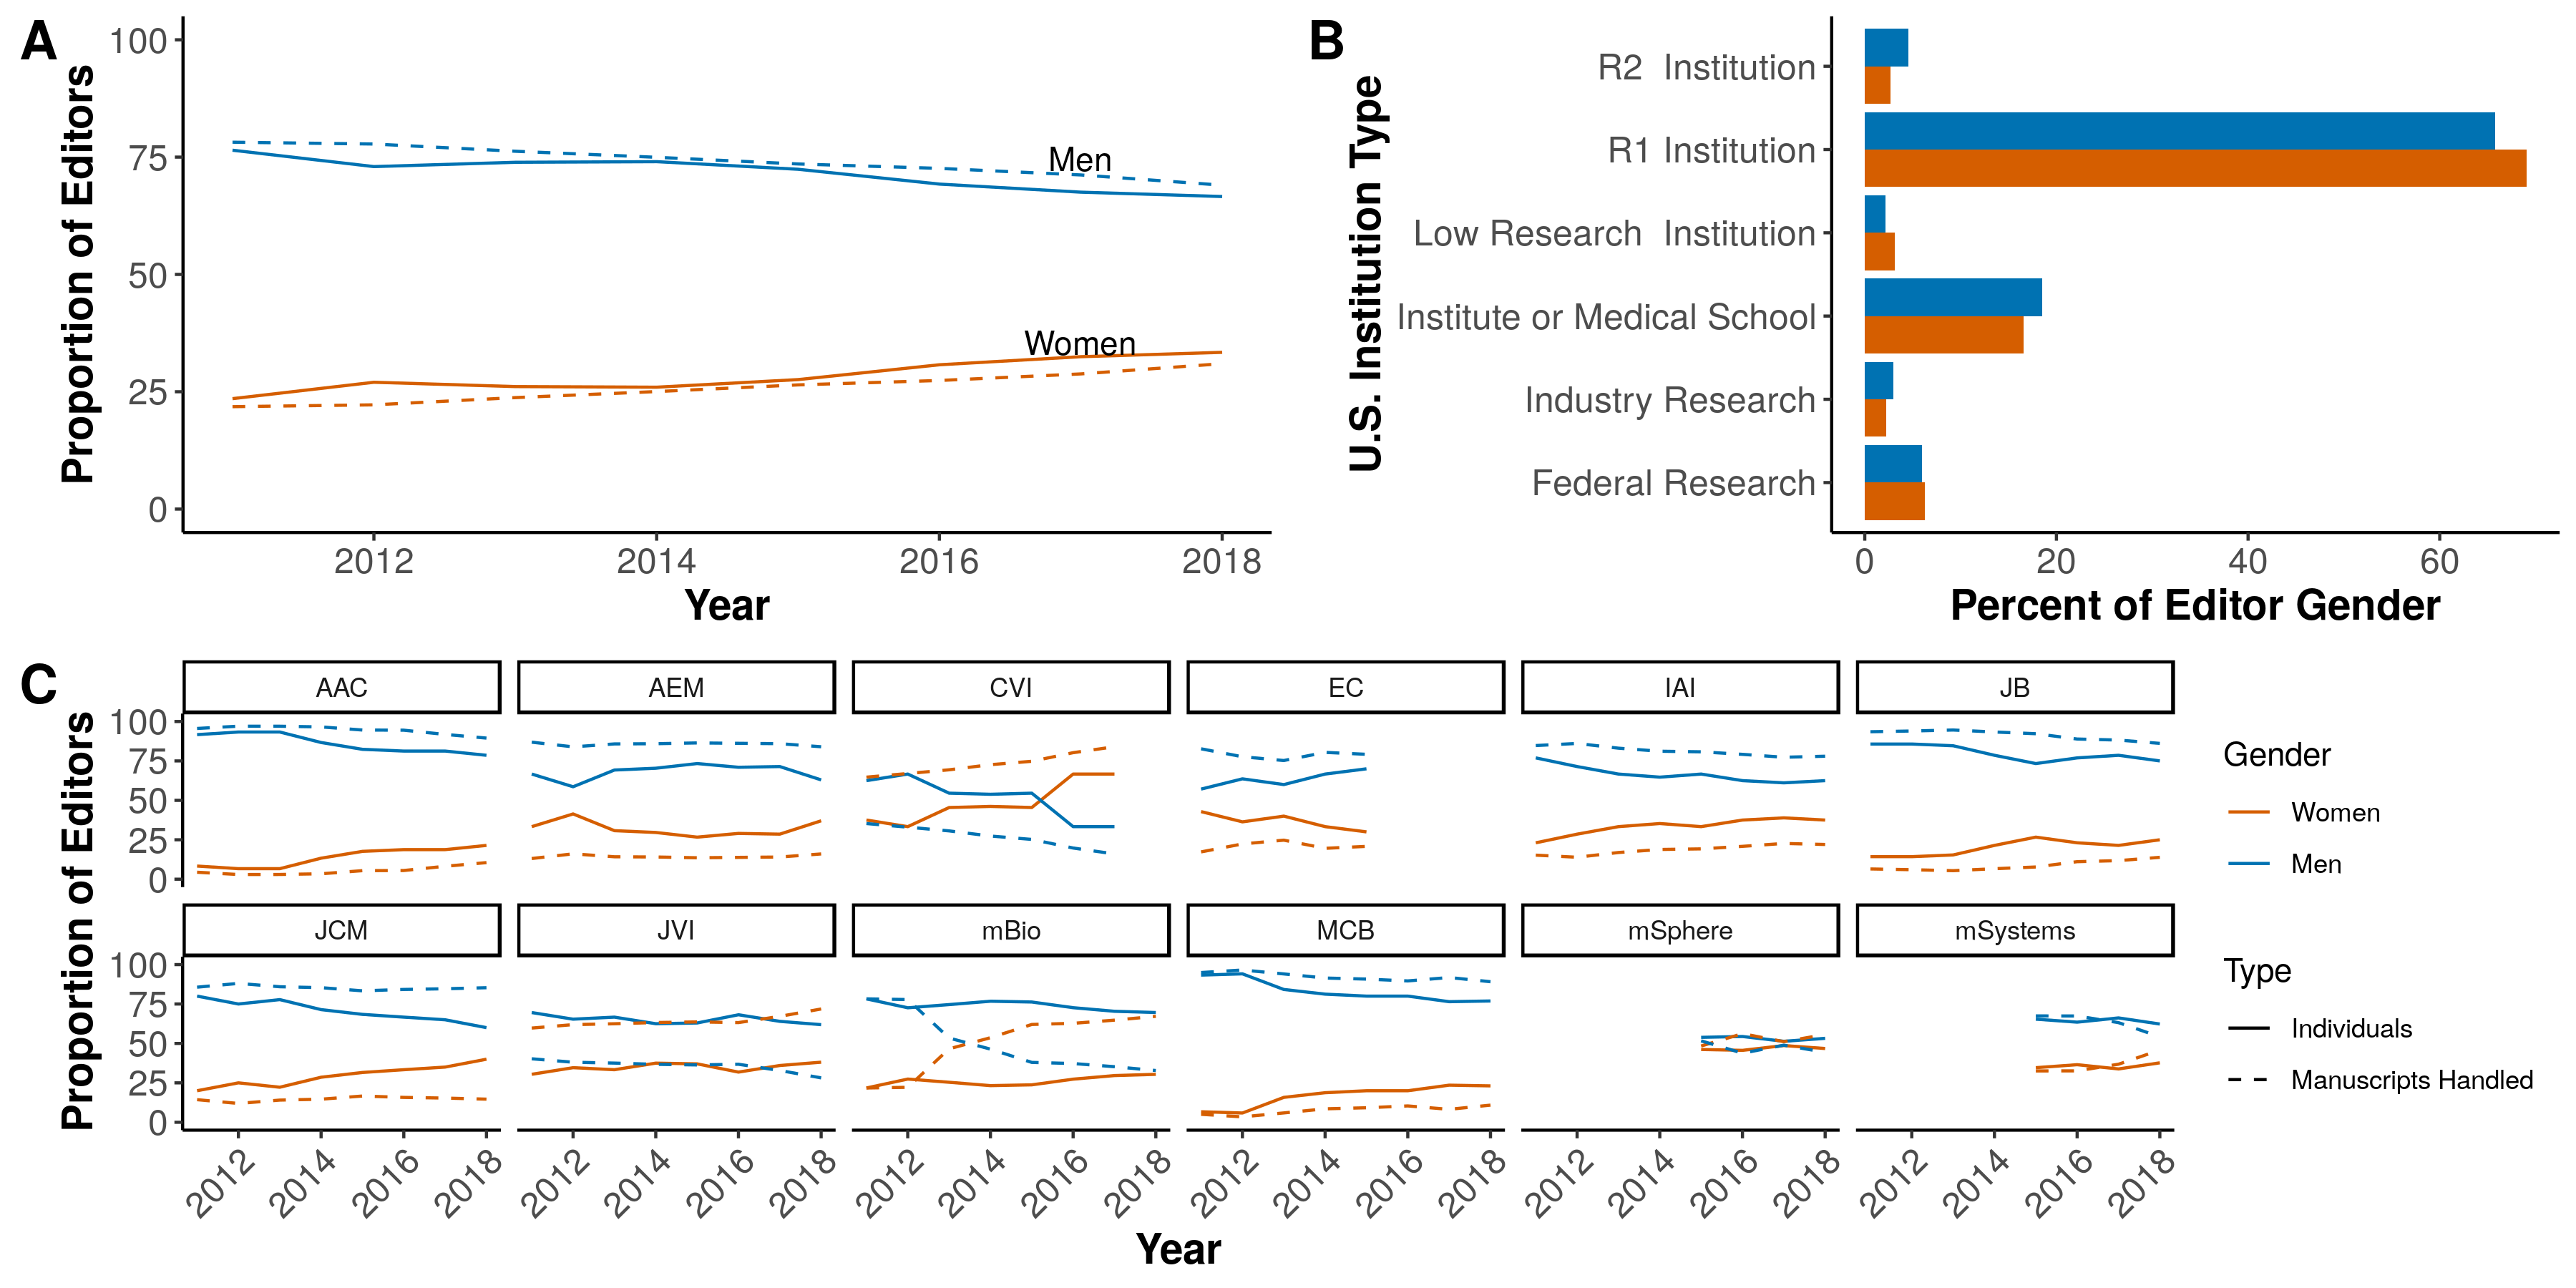
\includegraphics{Figure_1.png} \textbf{Figure 1. Gendered representation
among editors.} Proportion of editors (solid line) and their workload
(dashed lines) from 2012 to 2018. Data for men are blue, and women
orange. (A) All journals combined. (B) Breakdown by individual journals.
Editors and senior editors are pooled together, editorial rejections are
excluded. Each individual was counted once per calendar year. (C)
Percent of editors from each U.S. institution type by gender.

\textbf{Men dominate as gatekeepers and senior authors.} The term
gatekeepers collectively referres to those that facilitate the peer
review process, such as editors-in-chief (EIC), editors, and reviewers.
Between January 2012 and August 2018, ASM published 15 different
journals (), each of which has one editor-in-chief at a time. Two
journals, \emph{Eukaryotic Cell} (EC) and \emph{Clinical Vaccine
Immunology} (CVI) were retired during the period under study. In total,
there were X EICs, X\% of which were women. In 201X, the leadership of
CVI transferred from a man EIC, to a woman. The \emph{Journal of
Virology} (JVI) has had the same woman as EIC since 201X, while X review
journal has been led by a woman EIC since 201X. This study only examines
original research manuscripts, which eliminates three journals from the
remaining analyses (2 review journals and Genome Announcements).

In the remaining 12 journals studied, the total number of editors
(senior editors and editors pooled), was X and X\% were women. Over time
there has been a slow trend toward gender parity of editors (Fig. 1A,
solid lines), which is representative of senior editor trends. The
trends for each journal studied vary considerably, though most have slow
trends toward parity (Fig. 1B, solid lines). CVI and \emph{mSphere} are
the only ASM journals to have accomplished equal representation of both
genders, with CVI having a greater proportion of women editors than men
before it was retired. EC is the only journal with an increasing parity
gap.

To understand if men and women editors had proportionate workloads, we
calculated the percent of manuscripts handled by men and women editors,
not including editorial rejections. Across all journals, men handle a
slightly greater proportion of manuscripts (blue dashed) and women a
slightly smaller proportion (orange dashed), relative to their
respective editorial representations (Fig. 1A). This trend continues
accross most journals with varying degrees of difference between
workload and representation (Fig. 1B). There are exceptions. At
\emph{mBio} and \emph{mSphere}, workload and proportions are identical.
However, at CVI and JVI, the workload for women editors is much higher
than their representation, while the workload of men is considerably
less than their representation would suggest. In the years preceding its
retirement, the representation of women at CVI increased, which acted to
decrease the gap with their workload. However, representations and
relative workloads for men and women editors at JVI have held steady
over time.

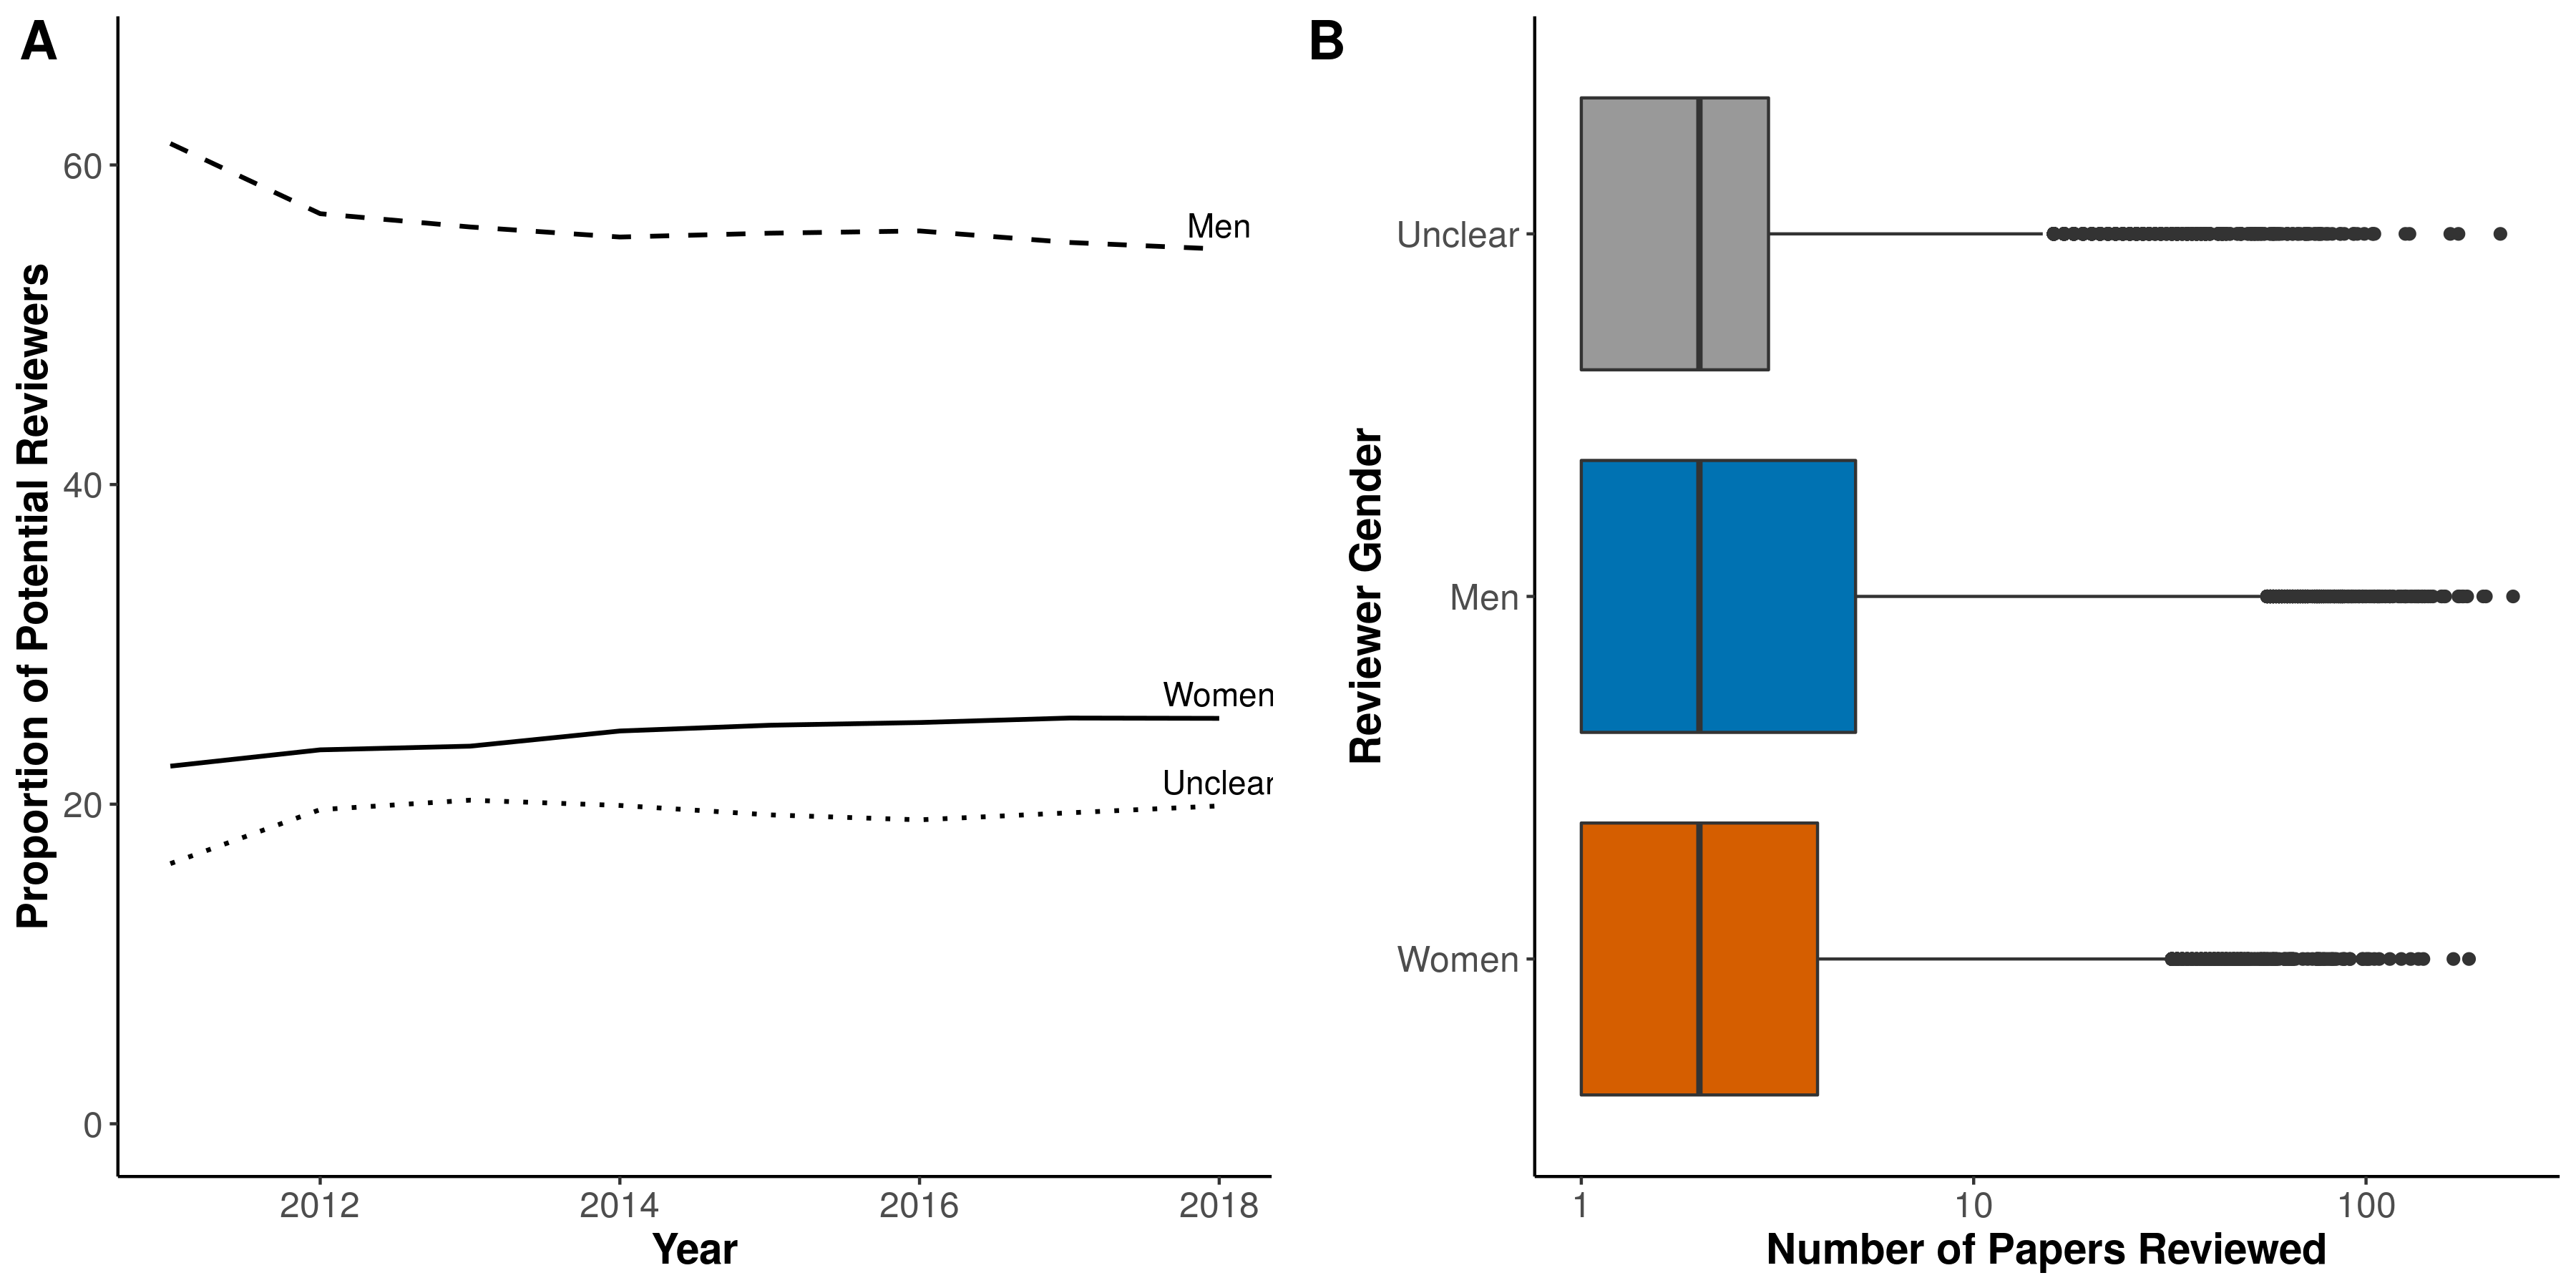
\includegraphics{Figure_2.png} \textbf{Figure 2. Reviewer
representation, workload, and response to requests to review.} (A)
Proportion of each gender listed as a possible reviewer from 2012 to
2018. (B) Comparison of total papers reviewed by each individual
according to gender. (C) Percent of each reviewer gender contacted to
review, according to the editor's gender. (D) The percent of reviewers
by gender that either accepted the opportunity to review or did not
respond to a request to review, split according to the editor's gender.
Reviewers were assigned one of three genders: men (blue/dashed), women
(orange/solid), or unknown (gray/dotted). Each individual was counted
once per calendar year. E) reviewer institution by gender

Given the relatively small number of editors at ASM journals (X), their
presenting genders where identified by hand while the genders of
reviewers and authors were predicted from their first names. Assigning
gender by first name resulted in 3 possible outcomes: men, women, and
unknown (when gender could not be assigned with confidence, see Methods
for validation). Over the time period studied, the proportions of each
gender have held steady among reviewers at ASM journals (Fig. 2A) and is
representative of both reviewer proportions at each journal, and the
potential reviewers at all journals combined (Fig. SX AB). The median
number of papers reviewed by individuals in each gender group is
equivalent (Fig. 2A). X, X, and X\% of men, women, and unknown reviewers
have reviewed only one manuscript. Editors of both genders contact
reviewers from all three gender groups at equivalent proportions, though
women editors contact more reviewers than men (Fig. 2C). This is likely
because reviewers of all genders, accept fewer, and ignore more,
requests to review from women editors than men (Fig. 2D).

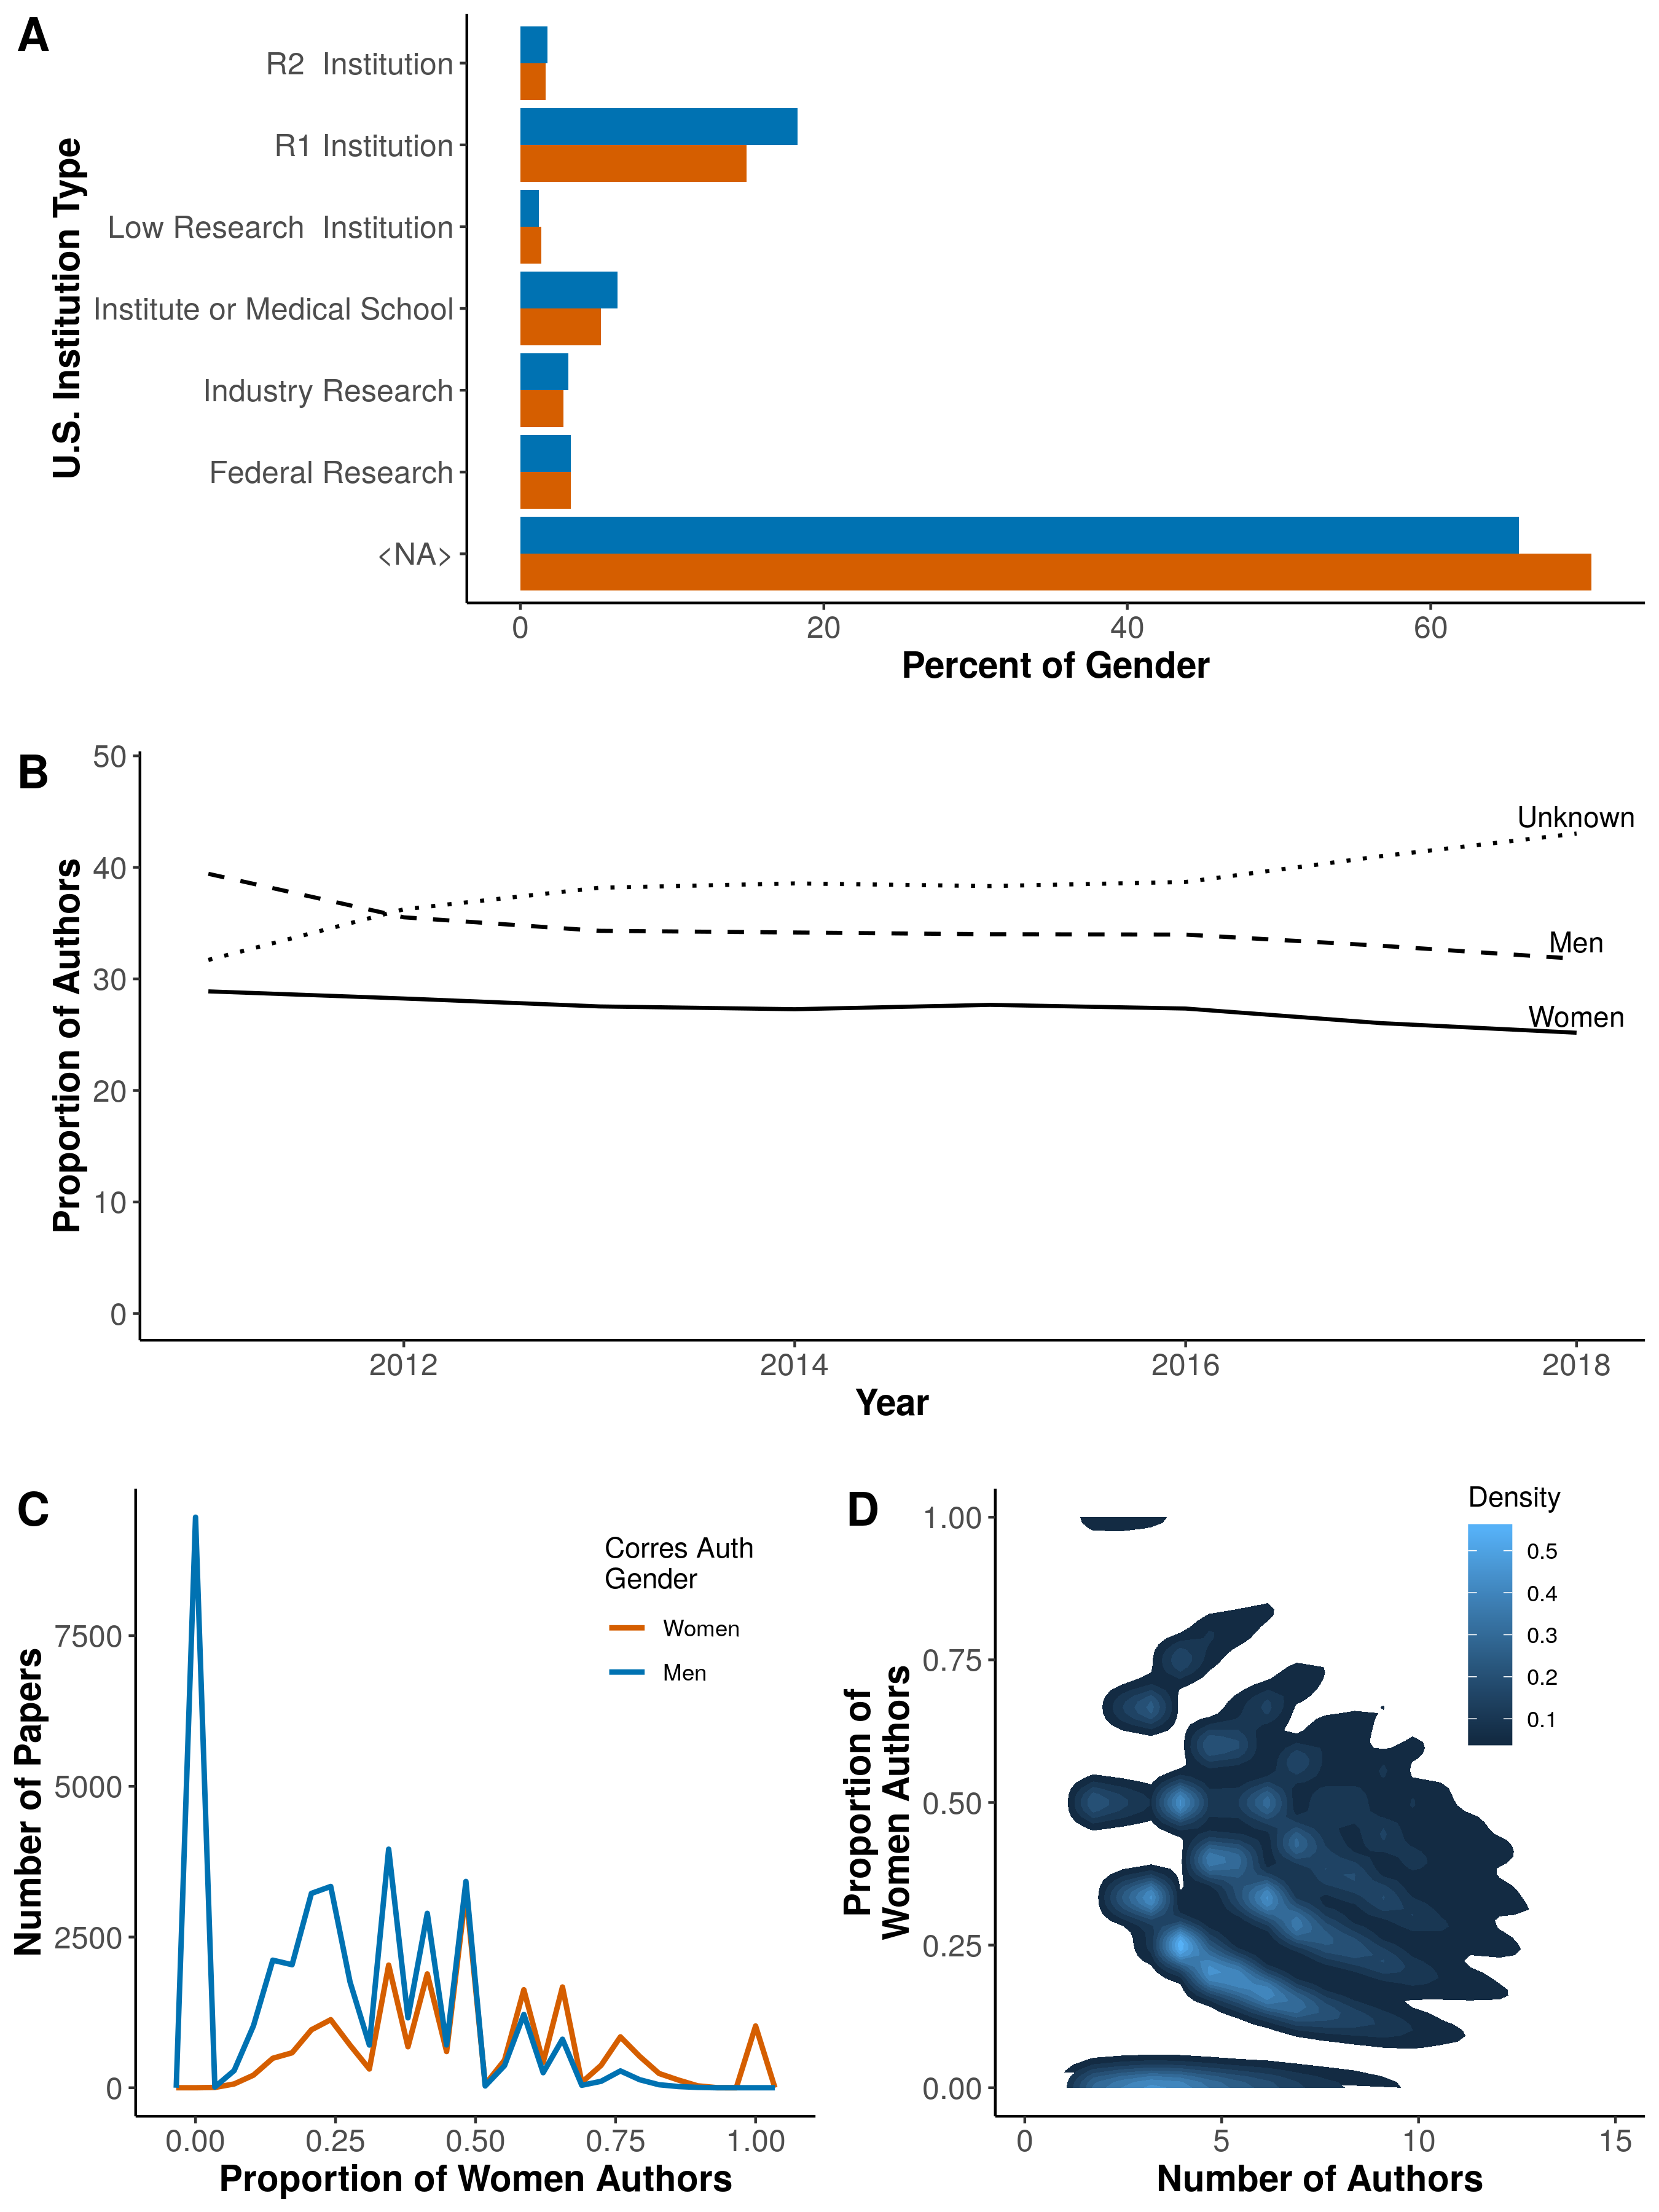
\includegraphics{Figure_3.png} \textbf{Figure 3. Author representation
by gender.} The proportion of (A) authors, (B) first authors, and (C)
corresponding authors from 2012 - 2018. (A, B) Solid lines indicate
individuals, dashed indicate proportion of manuscripts submitted. Men
indicated by blue and women by orange. All individuals counted once per
calendar year. The proportion of women authors on submitted papers
according to (D) the gender of the corresponding author or (E) the
number of authors. Unique manuscripts submitted from 2012 to 2018.

The proportions of men (long dash) and women (solid) authors at ASM have
decreased over time at equvalent rates, with a ratio of men to women
authors of 4:3 since 2012 (Fig. 3A). This decrease corresponds with an
increase in the proportion of unknown (dotted) authors. + Discuss author
\& inst stats -- split by author type? + Compare to global and ASM
membership stats + Globally - microbiology researchers are 60:40, M:F -
Elsevier + ASM membership - 38.37 (sept 2018)

X manuscripts submitted have men as corresponding authors but lack any
women authors. The number of papers submitted by women corresponding
authors with women comprising more than half of the authors exceeds
those submitted by men corresponding authors (Fig. 3X). Additionally,
the proportion of women authors decreases as the number of authors
increases (Fig. 3X). To verify that the trend is non-random, we ran a
logisitic regression model predicting the gender of the corresonding
author. Variables of the model included whether or not the corresponding
author's institution was in the U.S. or not, the total number of
authors, whether or not the article was published, the gender of senior
editors and editors, the number of revisions, and whether or not the
manuscript was editorially rejected. The value of the area under the
curve (AUC), for this model was 0.72, meaning that the model could
correctly predict gender 72 percent of the time. With a median weight of
4.09, the primary predictive driver of this model was the proportion of
women authors on a paper (even excluding single author and all men
author papers). All other variables had weights less than 1, indicating
they played no role in prediction of the corresponding author when the
proportion of women authors was present.

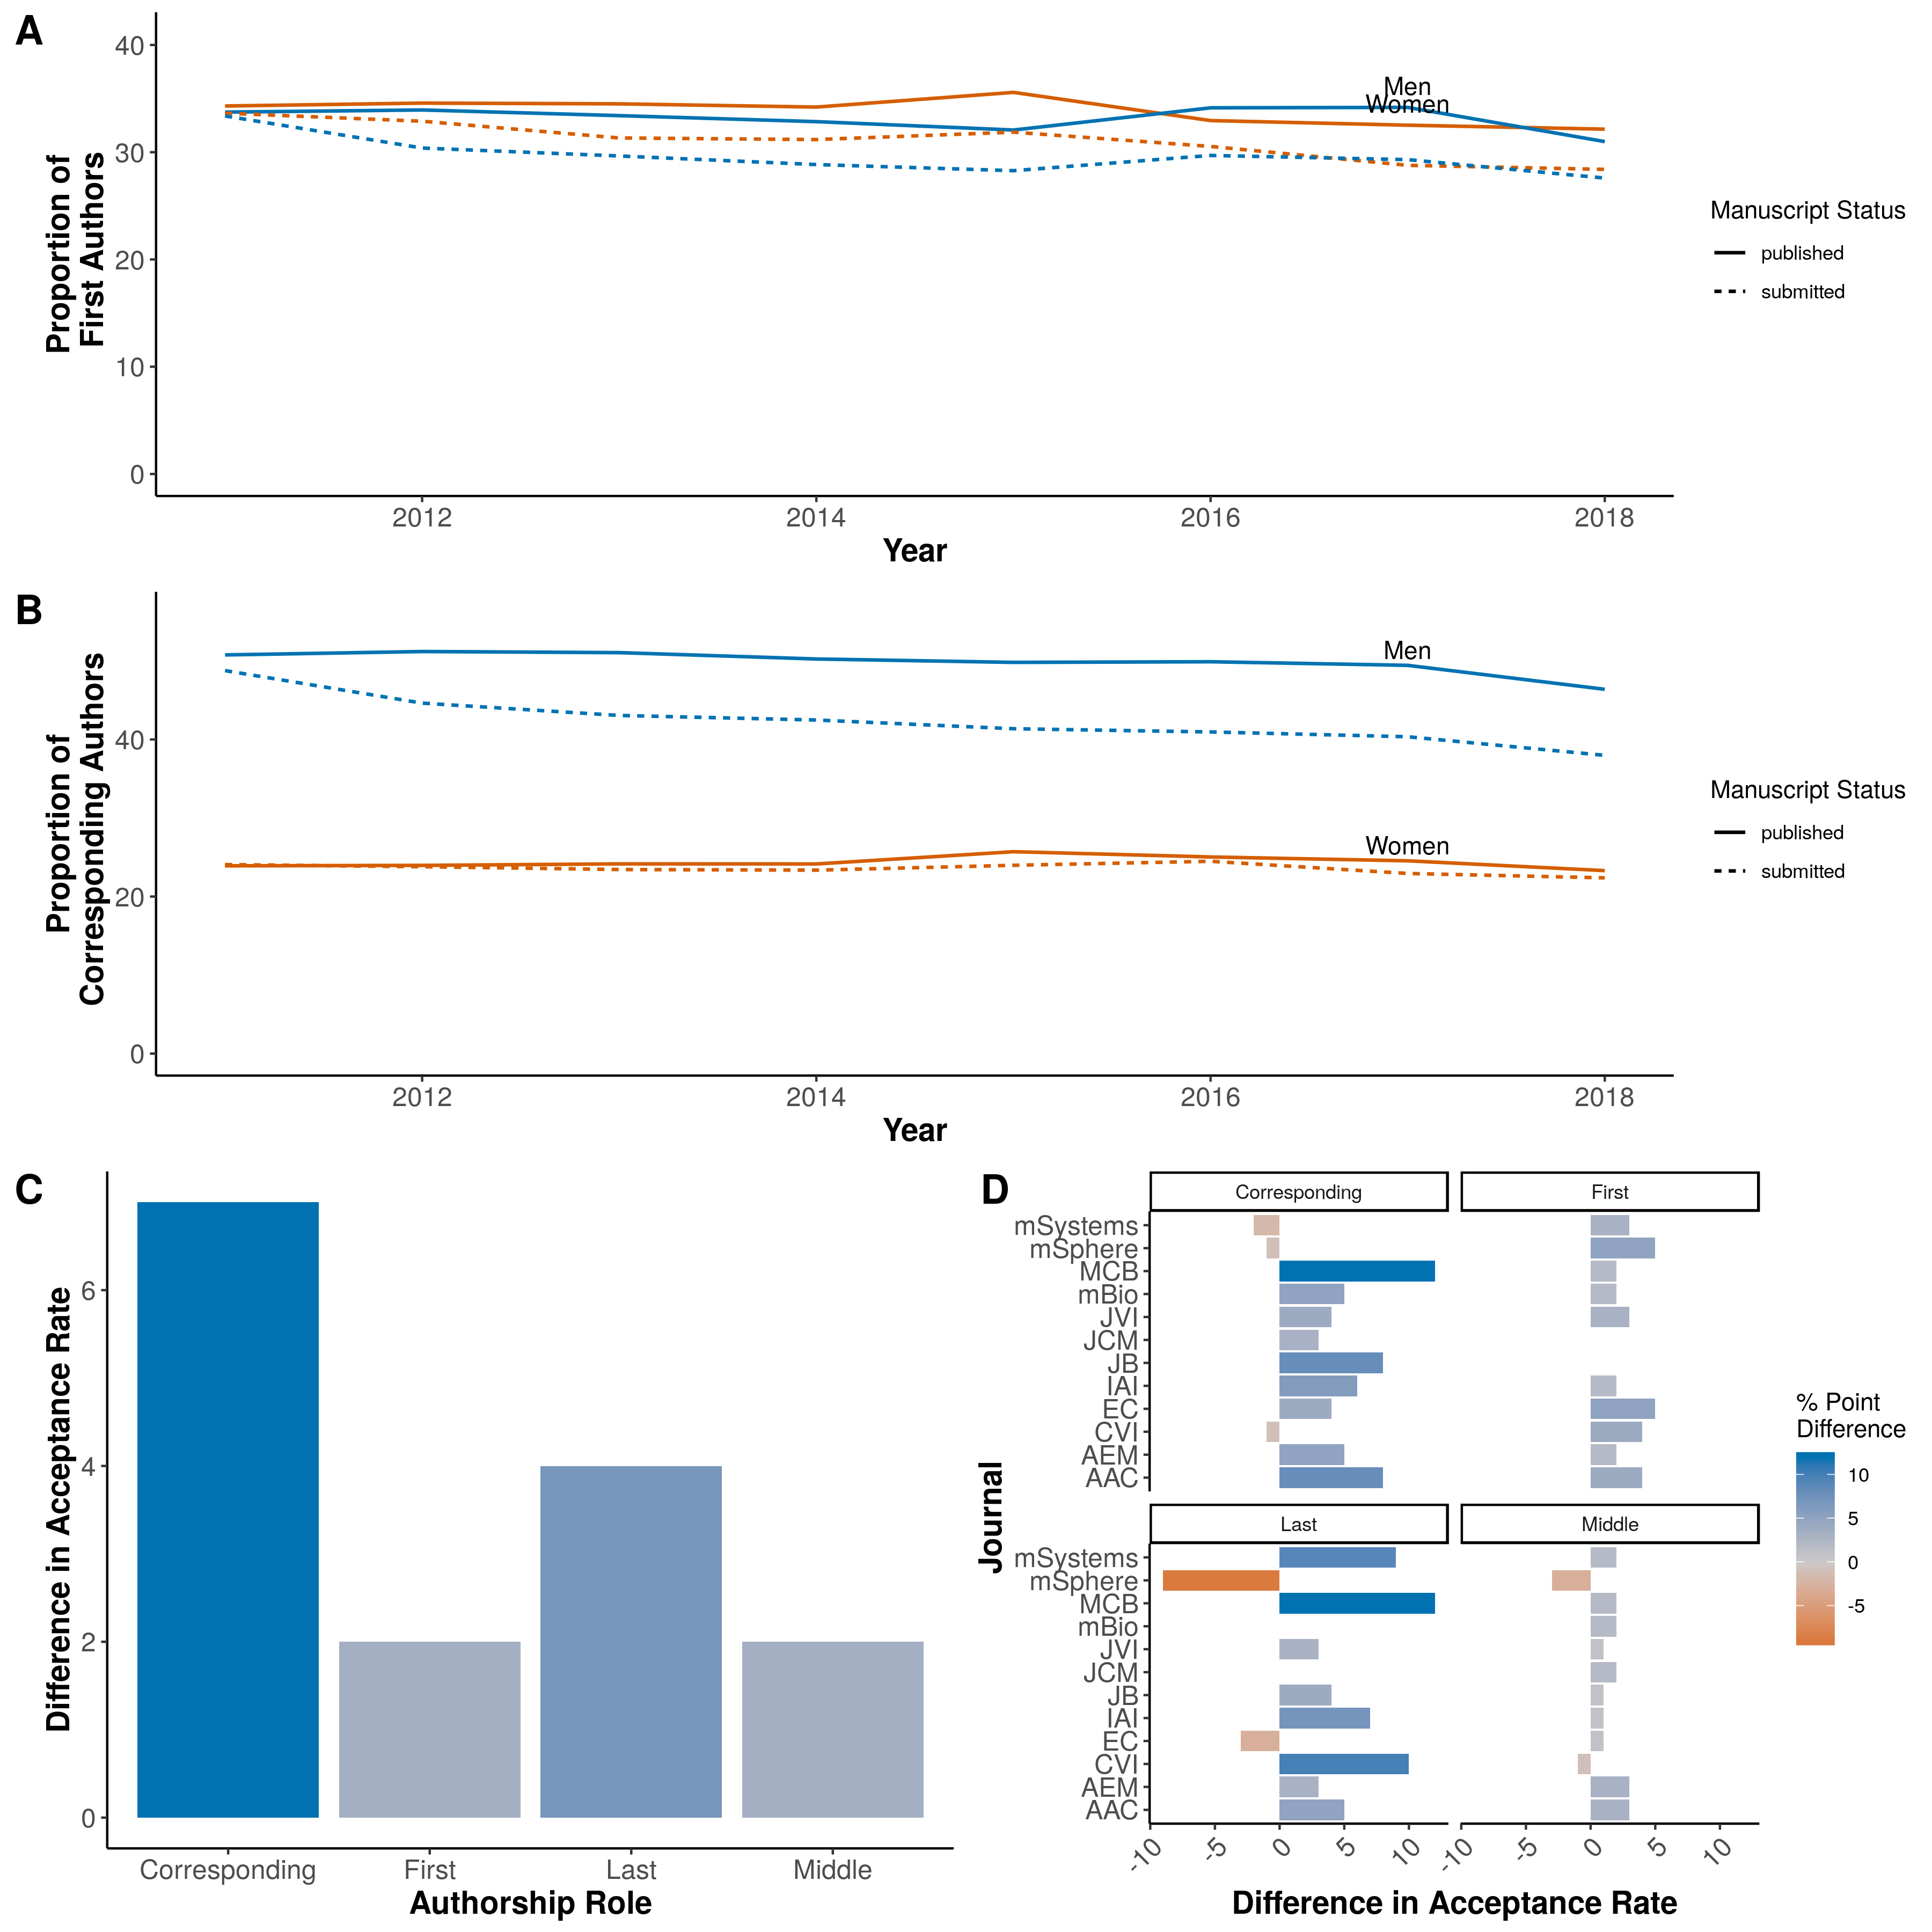
\includegraphics{Figure_4.png} \textbf{Figure 4. The difference in
percentage points of papers accepted} The proportion of (A) first
authors and (B) corresponding authors from 2012 - 2018. Solid lines
indicate individuals, dashed indicate proportion of manuscripts
submitted. Men indicated by blue and women by orange. The difference in
percentage points of papers accepted at (C) all journals or (D) for each
journal. Unique manuscripts were split according to the gender of the
corresponding, first, last, and middle author(s), and the acceptance
rate for each group calculated. The difference in acceptance rate was
determined by subtracting the acceptance rate of women-authored papers
from men-authored papers. The shade (ranging from orange to blue)
indicates the outperforming gender. No bar indicates no difference in
percentage points.

The proportion of papers submitted with men (blue dashed) and women
(orange dashed) first authors have remained constant and equivalent at
about 3X\% percent (Fig. 4A), as have their respective proportions of
published manuscripts (solid lines). Conversely, the proportion of
submitted papers with men corresponding authors has remained steady at
X\% and the proportion with women corresponding authors at X\%. However,
their respective proportions of published manuscripts are dissimilar
(Fig. 4B). The published manuscript proportion where men are
corresponding authors seems to have a much larger gap relative to that
of women corresponding authors. These trends are similar across
individual journals (Fig. SX).

We wanted to know whether the increase in published proportions are
proportionally equivalent for men and women corresponding authors or if
this was evidence for disproportionate success by men relative to women.
To answer this question, we calculated the difference in percentage
points between a given outcome for men and women, e.g., the percentage
point difference in acceptance rates is the acceptance rate for men
minus the acceptance rate for women. A positive value indicates that men
receive the outcome more often than women, whereas a negative value
indicates that women outperform men in the given metric. To correct for
the large disparity in the participation of women relative to men at ASM
journals, all percentage point comparisions are made relative to the
gender and population in question. First, we calculated the difference
in acceptance rate percentage points for men and women at each author
type (e.g., corresponding, first, last, and middle). Men outperformed
women in all authorship roles across ASM journals combined, with the
greatest difference seen for corresponding authors with a difference of
X percentage points (Fig. 4C). When broken down by journals, there is a
clear trend to overperformance by men in both corresponding and last
authorship categories, with some exceptions (Fig. 4D). The primary
exception is \emph{mSphere}, where papers with a woman last author are
accepted almost 10 percentage points more than those with a man as last
author.

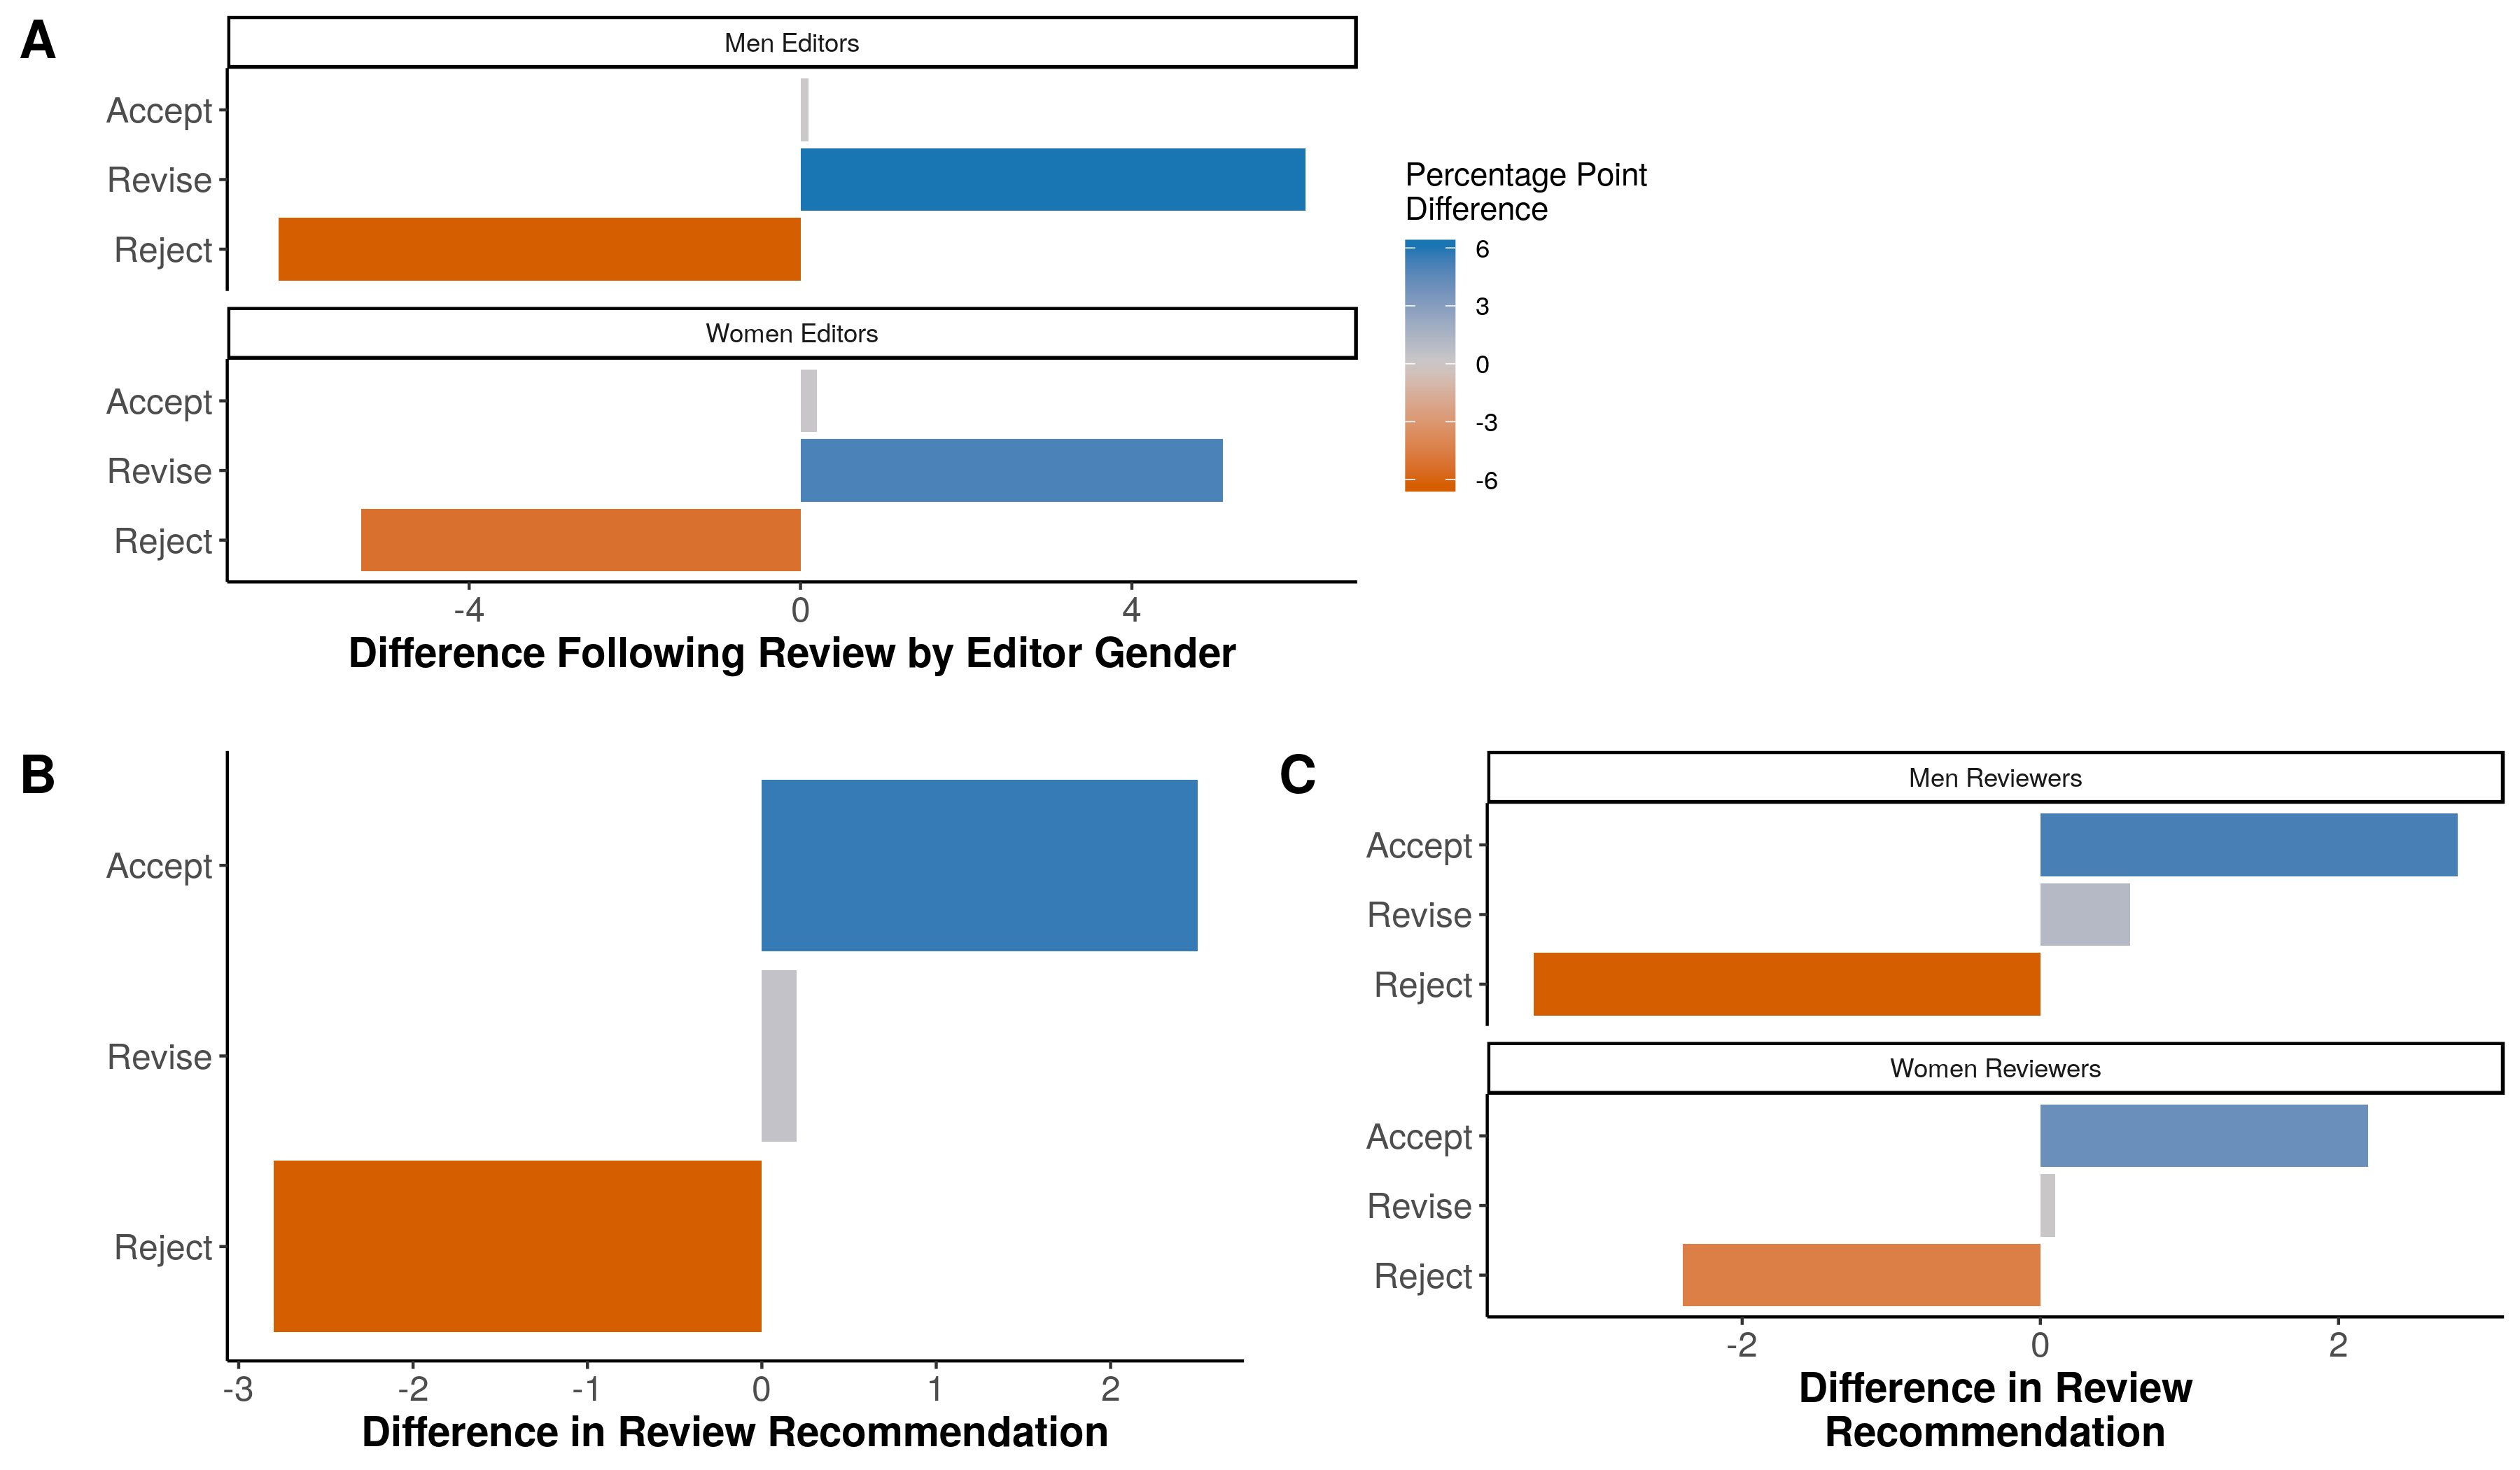
\includegraphics{Figure_5.png} \textbf{Figure 5. Difference in rejection
rates by author gender.} The percent of manuscripts rejected by author
gender and type (e.g., corresponding, first, last, middle) at (A) all
journals combined or at (B) each journal, which shows the difference in
percent rejection rates. (C) The difference in percent editorial
rejection rates at each journal, vertical line indicates the difference
for all journals combined. (D) The difference in percentage points
between each decision type following the first peer review, vertical
lines indicate the difference value for all journals combined. The
difference in rejection rates was determined by subtracting the
rejection rate of women-authored papers from men-authored papers within
each category. The shade (ranging from orange to blue) indicates the
outperforming gender. No bar indicates no difference in percentange
points.

\textbf{Papers submitted by women have more negative outcomes than those
submitted by men.} To better understand the percentage point difference
in gendered performance (Fig. 4), we next compared the rejection rates
at each author stage. While middle and first authors were rejected at
similar rates for men and women, senior woman-authored (e.g.,
corresponding, last) manuscripts are rejected more frequently than those
authored by men (Fig. 5A). Breaking it down by individual journals,
there are several instances where the overall trend is repeated or even
amplified (e.g., AAC, IAI, JB, \emph{mBio}, MCB) (Fig. 5B). The greatest
effect was observed when comparing the gender of corresponding authors,
so we used this sub-population to further examine the difference in
acceptance/rejection rates.

We next compared the rejection rates for men and women corresponding
authors at two different bottlenecks, before and after the first peer
review. Many papers are immediately rejected by editors/EICs instead of
being sent to peer review, often due to issues of scope or percieved
quality. We refer to these as editorial rejections. Alternately, editors
could send papers out for review by two or three experts in the field,
or peers. The reviewers make suggestions to the editor who decides
whether the manuscript in question should be accepted, rejected, or sent
back for revision. At ASM journals, manuscripts with suggested revisions
that are expected to take more than 30 days are rejected, but generally
encouraged to resubmit. Papers authored by women are editorially
rejected as much as 12 percentage points more often than those authored
by men (Fig. 5C). The percentage point difference at all ASM journals
combined is -3.X (vertical line), and two journals, MCB and \emph{mBio},
have more extreme percentage point differences. Papers authored by men
and women are equally likely to be accepted after the first round of
review (Fig. 5D, right panel). However, women-authored papers are more
likely to be rejected (left panel) while men-authored papers are more
often given revision decisions (center panel). Three journals, JB, AAC,
and MCB, have percentage point differences in rejection and revision
decisions that are more extreme than for all ASM journals combined (+/-
X\%, vertical line).

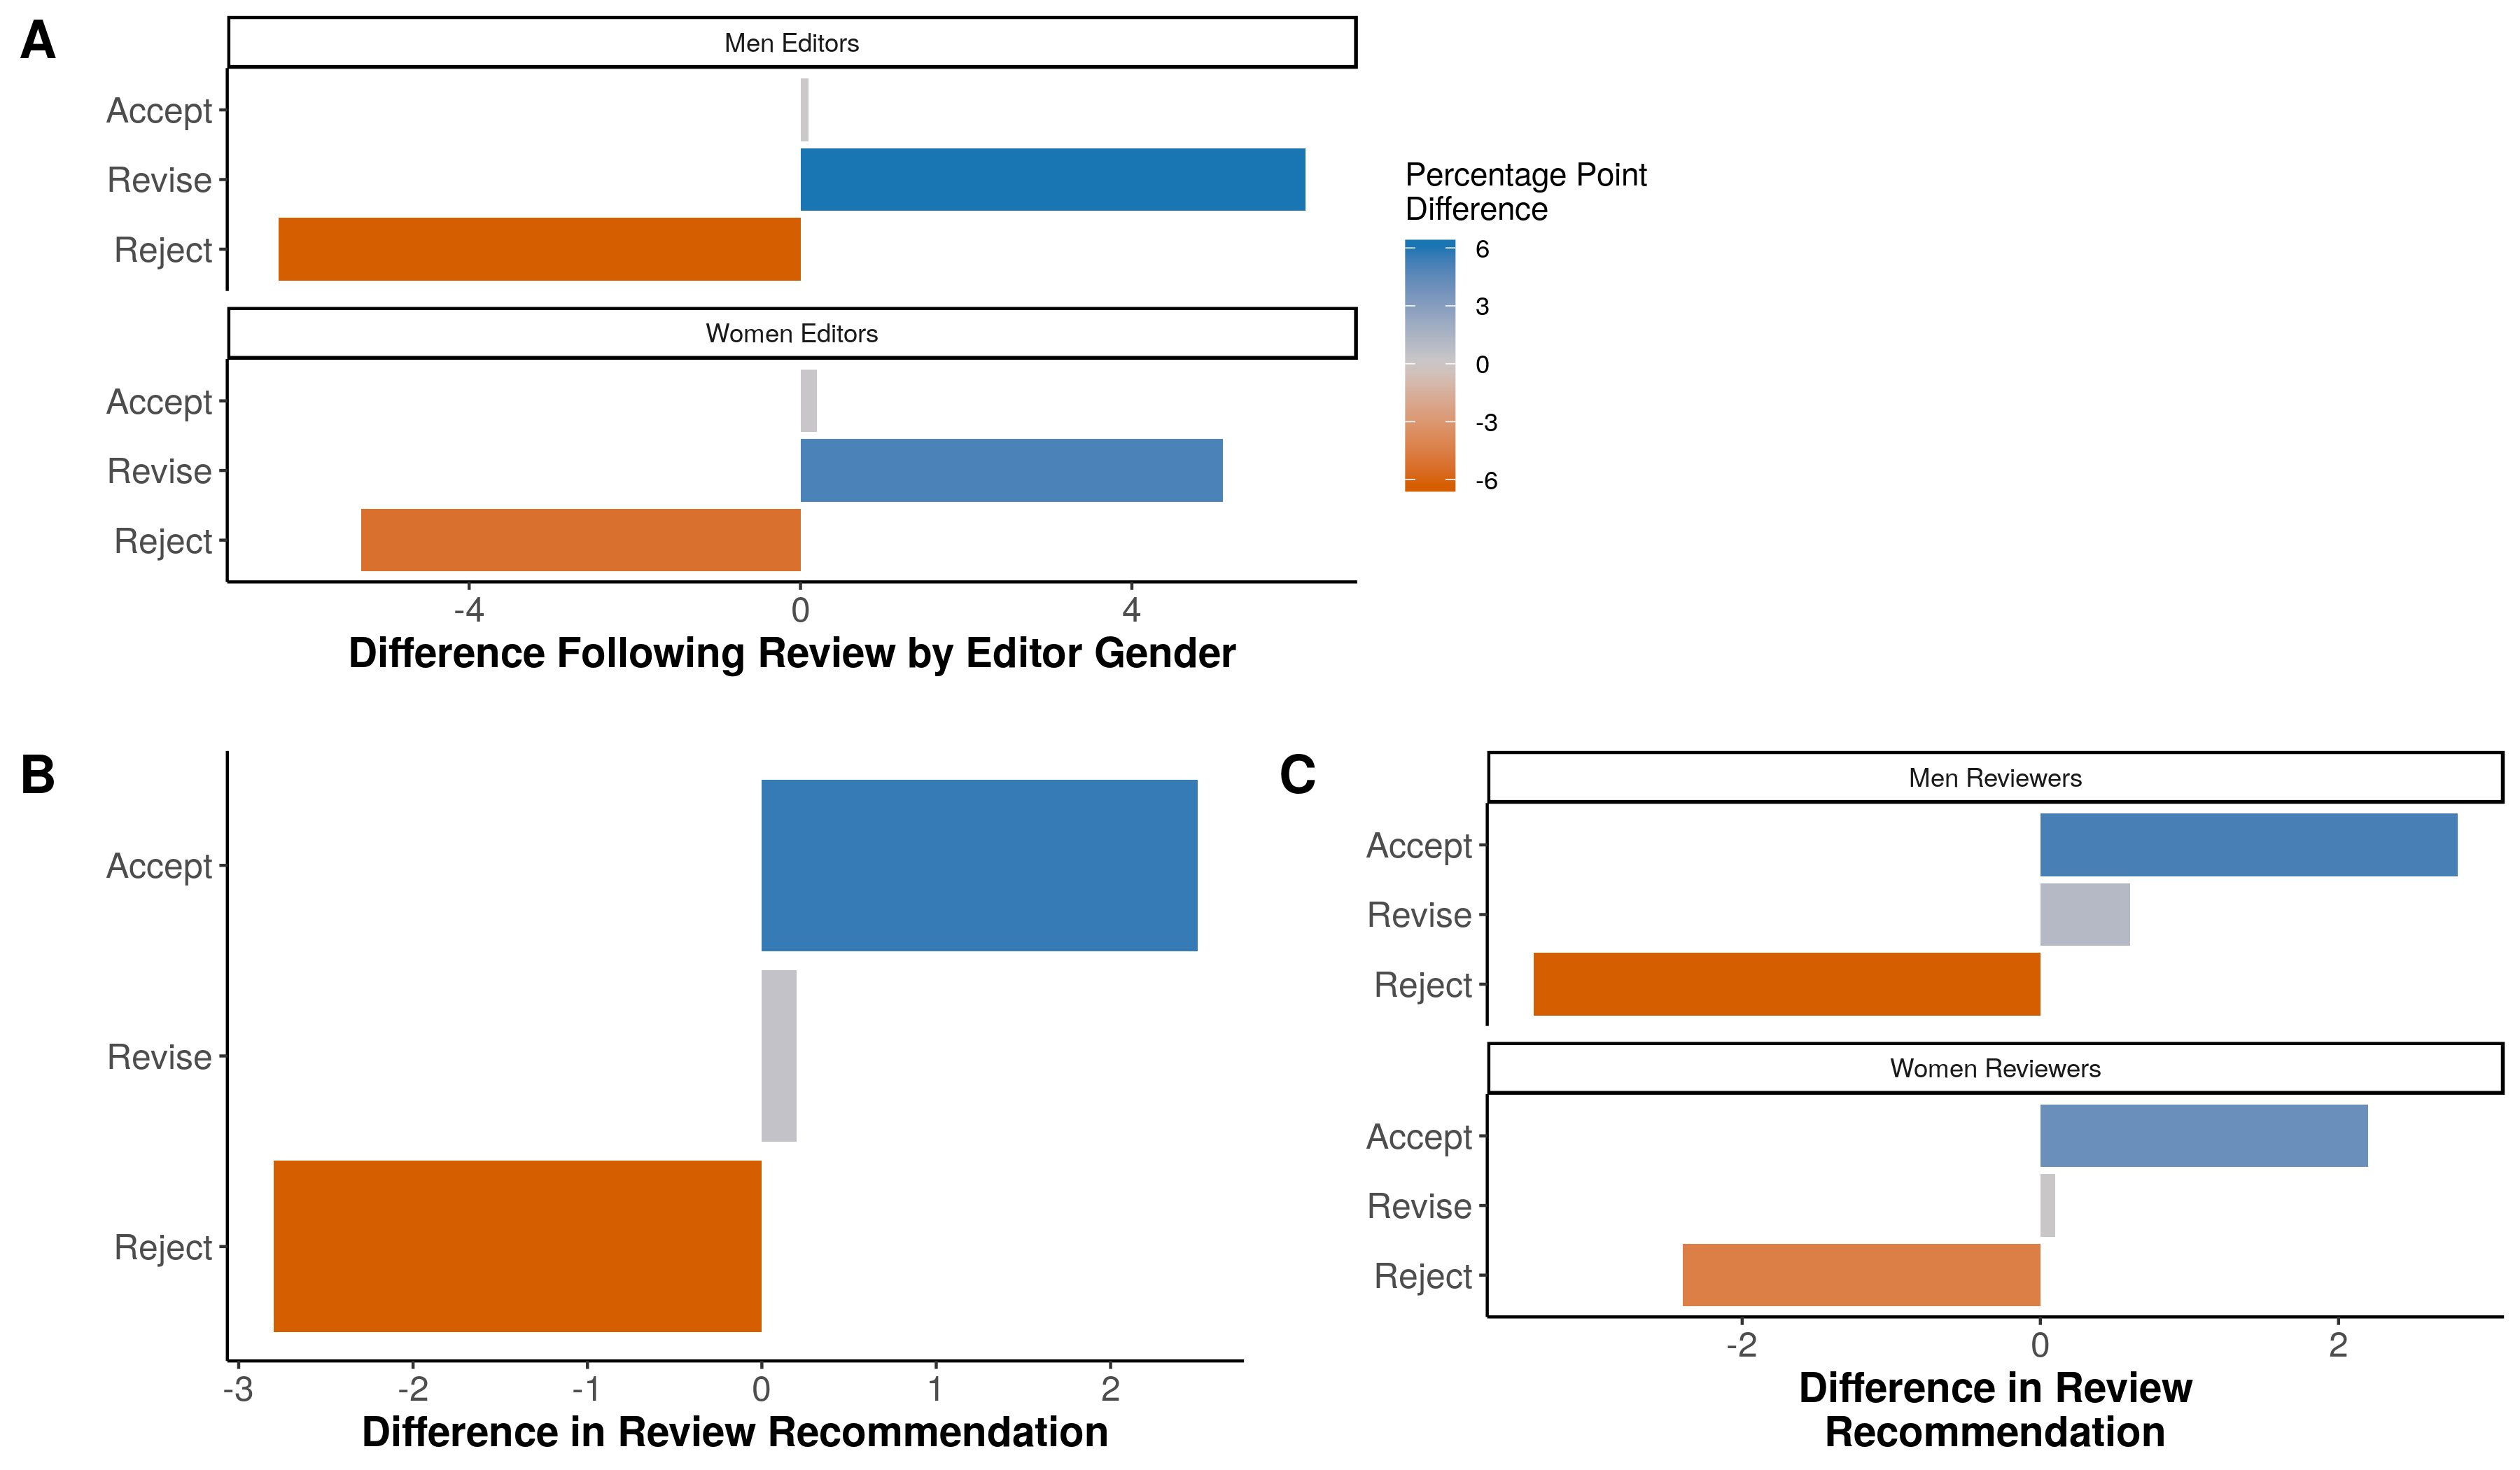
\includegraphics{Figure_6.png} \textbf{Figure 6. Difference in decisions
or recomendations according to the gatekeeper gender.} (A) Effect of
editor gender on the difference in percentage points for decisions
following review at all journals combined. (B) Difference in percentage
points for review recommendations and (C) how that is affected by
reviewer gender.

We next wanted to understand how gatekeeper (editor/reviewer) genders
influenced the outcomes observed in Fig. 5D. Both men and women editors
reject proportionally more women-authored papers, with men editors
making revise decisions on papers authored by men more often than those
authored by women (Fig. 6A). Reviewers are more likely to suggest
rejections for women as compared to men, though no difference in revise
suggestions were observed (Fig. 6B). Both men and women reviewers
recommended rejection more often for women-authored manuscripts though
only men reccomended acceptance more often for men-authored manuscripts
(Fig. 6C). Women reviewers suggested revision on women-authored papers
more often than men-authored manuscripts.

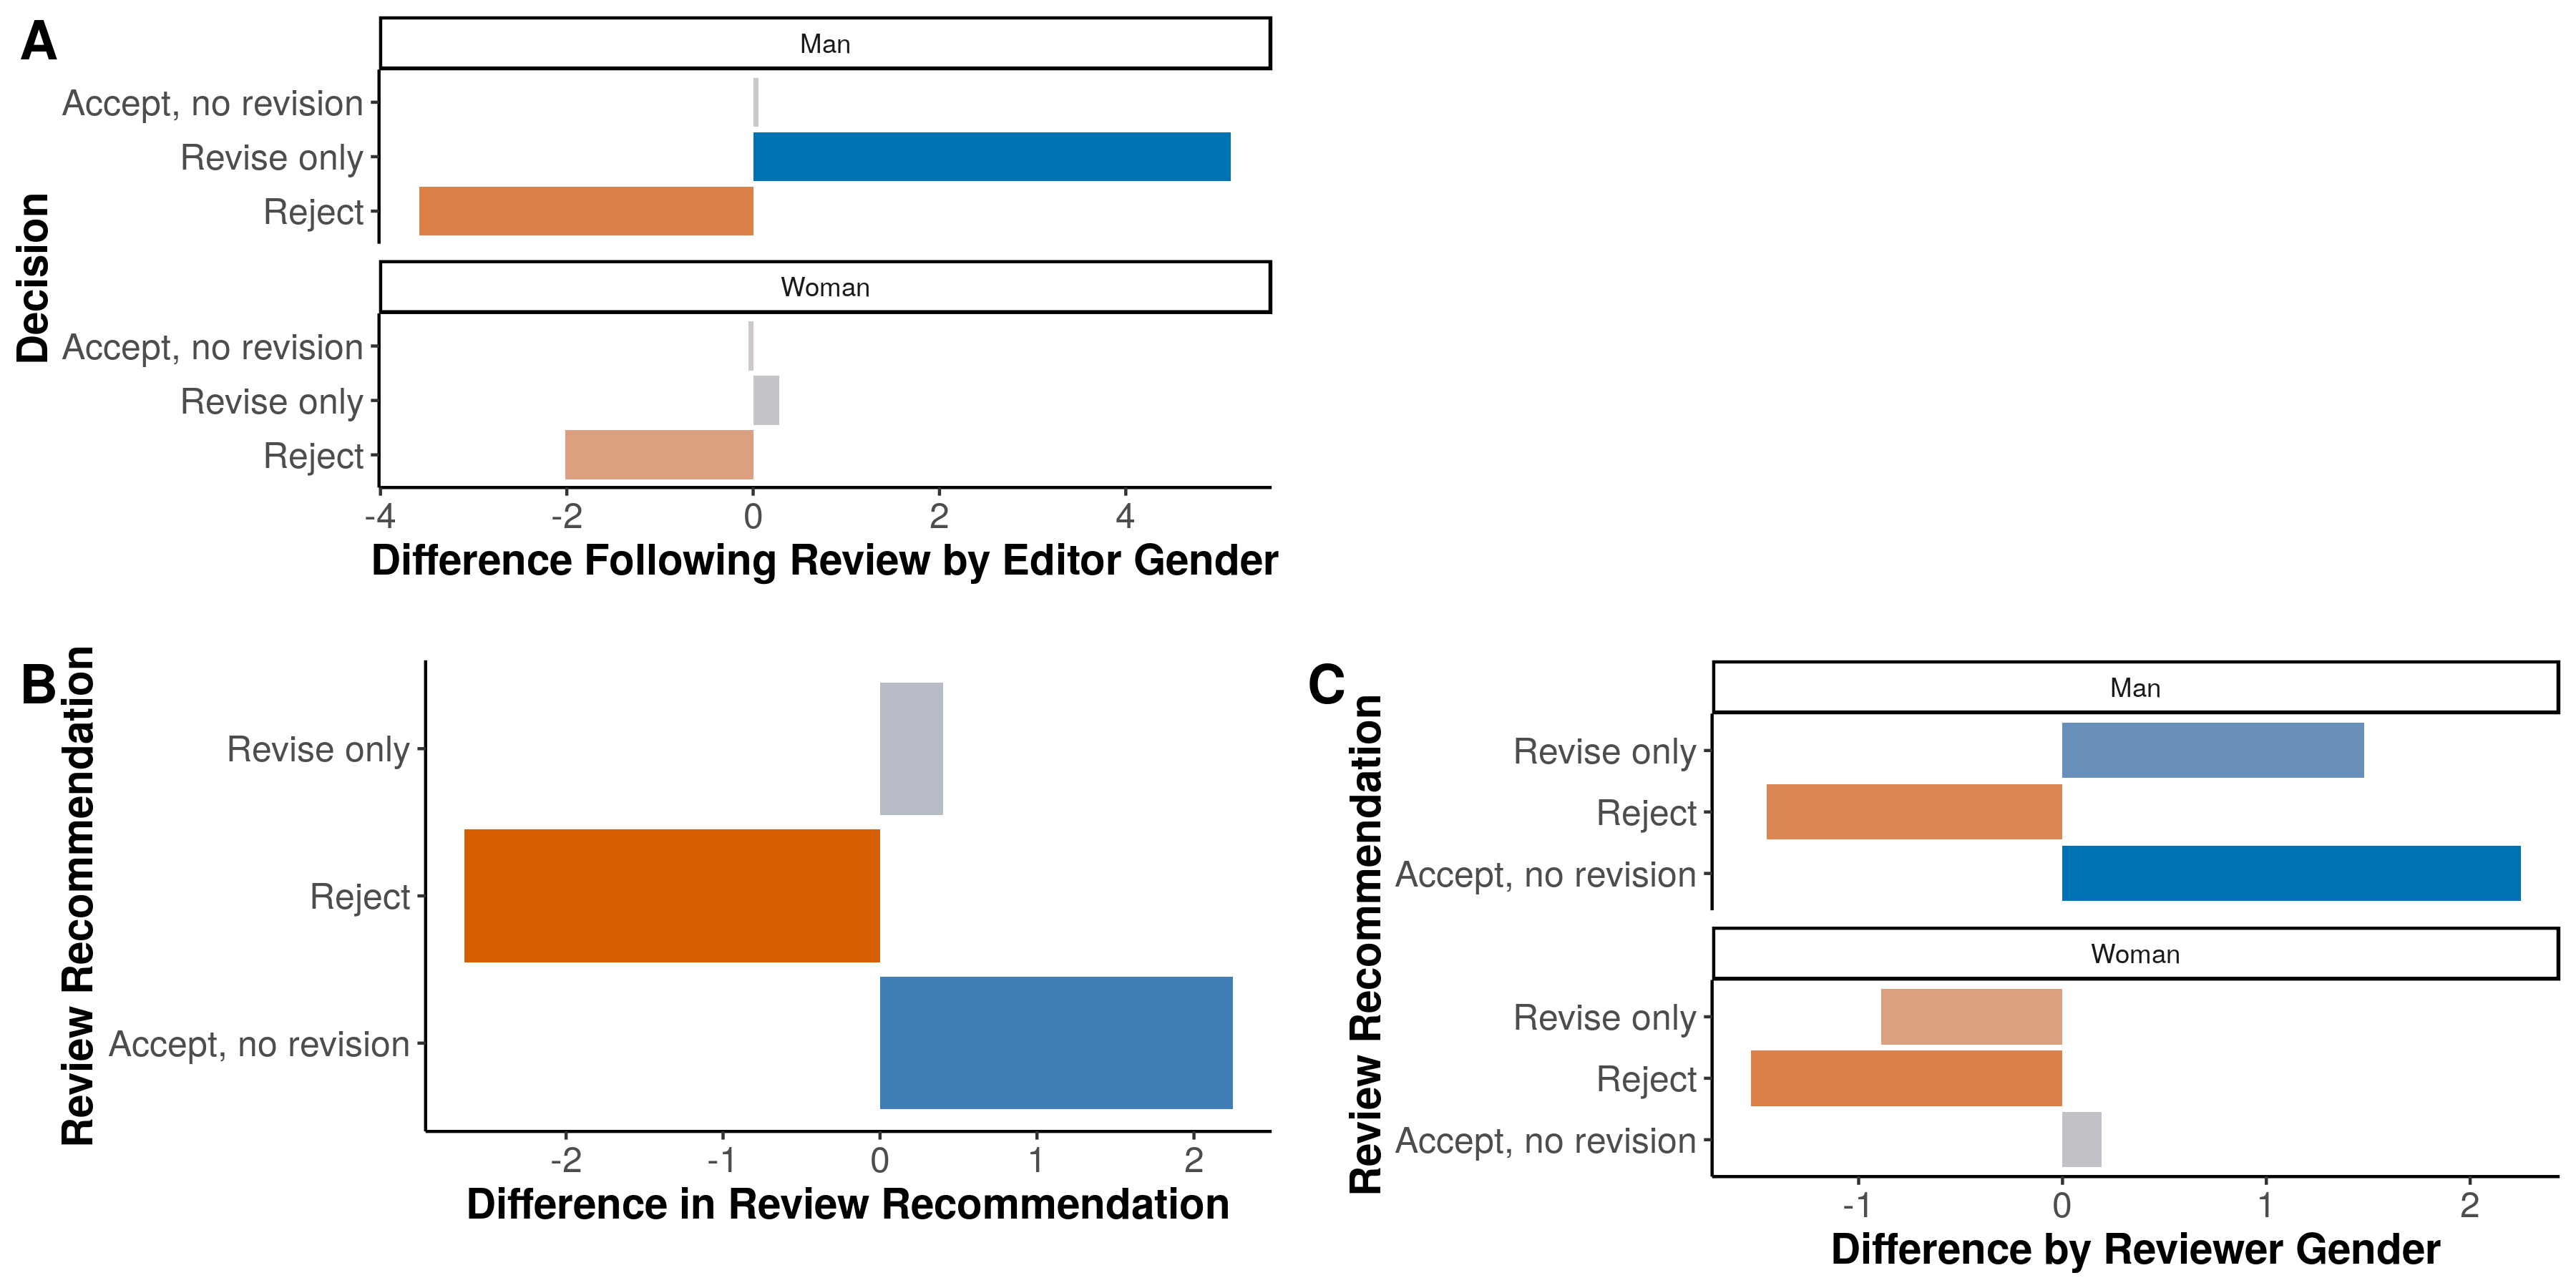
\includegraphics{Figure_7.png} \textbf{Figure 7. Impact of origin and
U.S. institution type on manuscript decisions by gender.} Difference in
percentage points for corresponding authors in the U.S. (A) editorial
rejections, (B) following first review, and by U.S. institution types
(C) acceptance and editorial rejections (D) acceptance decisions
according to editor gender.

\textbf{Multiple factors contribute to overperformance by men.} The high
rejection rate for the unknown population suggested that there may be
additional complications due to geography and prestige bias is a
well-established phenomenon. To try to separate these factors affect
manuscript decisions among corresponding authors, we next looked at the
outcome of papers submitted by authors at US institutions. + slight
disparity in editorial rejection \& acceptance rates according to
institution type (rej\_by\_inst\_type.R) + greatest difference (4\%)
occurs for institute/medical schools + trend holds for most journals and
is \textgreater{}20\% diff at JCM (R2s), mBio (Federal), MCB (low
research), AEM (industry research) (Supplementary\_A) + men from
institutes/medical schools outperform women \textgreater{}7\% for
acceptance across all journals + \textgreater{}20\% in favor of men at:
EC (fed researh), mSphere \& JVI (Low research), AEM \& MCB (industry
research), JCM/JB/JCM (R2 institution) (Supplementary\_B) + women
editors highly favor men from medical schools, slightly favor men from
R2 \& industry -- what is the n? + men editors favor men from R1, R2 and
medical schools, slightly favor women from low \& industry research --
what is the n? + rev\_score\_analysis.R + men at R1, low research,
medical schools \& fed research are favored by reviewers over women (B)
+ reviewer\_gender\_analysis.R + women reviewers are more likely to
recommend acceptance for women from low research \& federal institutions
(D) + women reviewers are more likely to recommend acceptance for men
from R1 \& industry instutitions (C) + men are more likely to recommend
acceptance for women from R2 institutions \& favor men from R1 \&
medical institutes (D)

\begin{itemize}
\tightlist
\item
  logistic regression data
\item
  discipline clusters -- \%F \&/or \%point diff
\end{itemize}

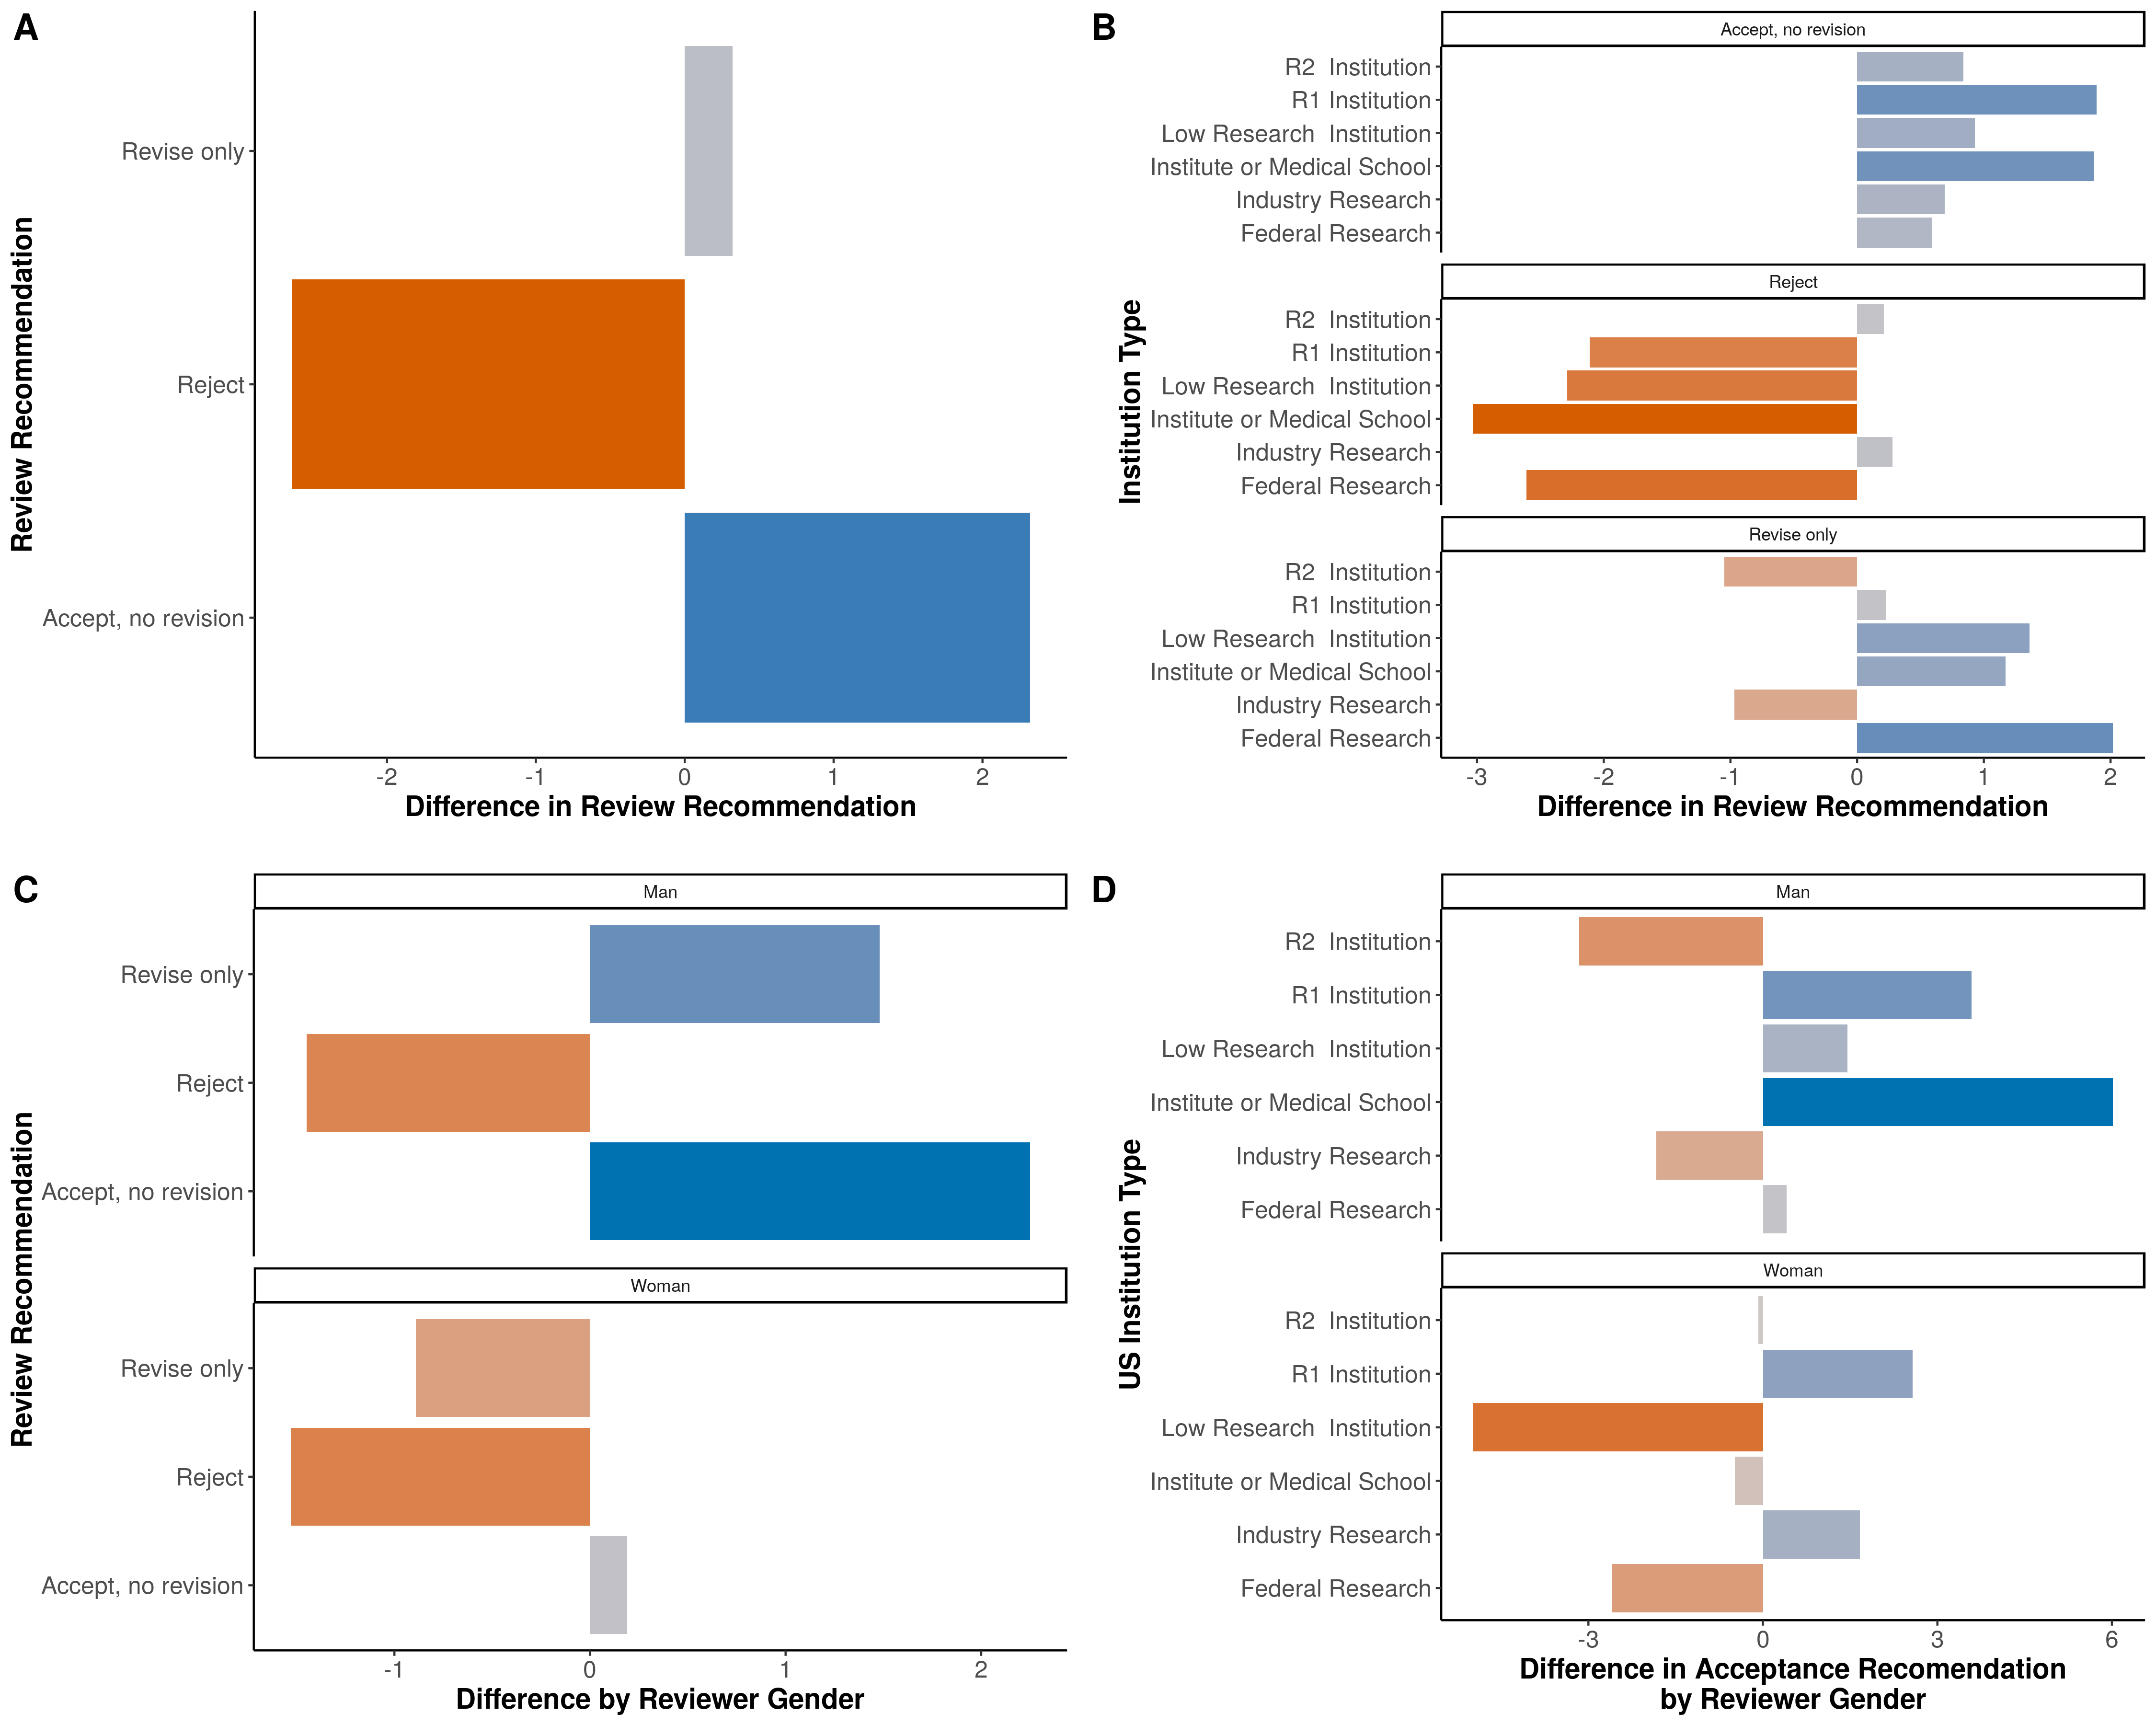
\includegraphics{Figure_8.png}

\textbf{Figure 8. Comparison of time to final decision and impact by
gender.} The number days (A) between when a manuscript is initally
submitted then finally published and (B) that a manuscript spends in the
ASM peer review system. How the impact of papers published by men (blue)
versus women (orange) vary according to (C) cites and (D) total reads.
Citation data includes articles published between 36 and 48 months prior
to August 2018. Total reads includes both HTML and PDF online views for
articles published between 12 and 24 months prior to August 2018. Impact
data are divided by the number of months published.

\textbf{Percieved competency compounds the low representation of women
authors.} In addition to manuscript decisions, other disparate outcomes
may occur during, or after, the peer review process. To determine
whether women-authored papers spent more time between being submitted
and ready for publication, we compared the number of revisions, days
spent in the ASM peer review system, and the number of days from
submission to ready for publication to those authored by men. Papers
authored by women take slightly longer (from submission to ready for
publication) than men at some journals ( \emph{mSphere}, \emph{mBio},
\emph{mSystems}, CVI, JB, JCM, AEM) despite spending similar amounts of
time in the ASM journal peer review system (Fig. 8AB), and having
\textbf{similar revisions prior to acceptance-add to supp}
(Supplementary\_C). Papers rejected following review that were submitted
by women do not generally take longer (in days) to be rejected, or have
more revisions (Fig. SX).

The peer review process does not end when a manuscript is published.
Instead, it is the continuation of the cyclical and self-reinforcing
nature of publishing. Published manuscripts are cited and used to build
future research and publications. The number of citations a manuscript
recieves has implications for both science and research careers since
they amplify visibility of an idea and its author(s). To understand if
papers published at ASM journals have differing impacts based on the
gender of their corresponding author, we compared paper citations to
reads. Women-author papers tend to receive lower cites per month
published than those authored by men, despite equivalent internet reads
(e.g., HTML, PDF, and abstract views).

Some consider a journals impact factor to be a proxy measurement of a
paper's quality. Previous research has found that women are less likely
to be published in high impact factors, despite gender parity in the
field. To determine if this was the case at ASM journals, we compared
how often men and women corresponding authors submitted to two broad
scope microbiology journals with differing impact factors. We found that
while women submit to both higher and lower journals at similar rates,
women are more highly represented in the lower impact journal.
\textbf{add numbers/stats}

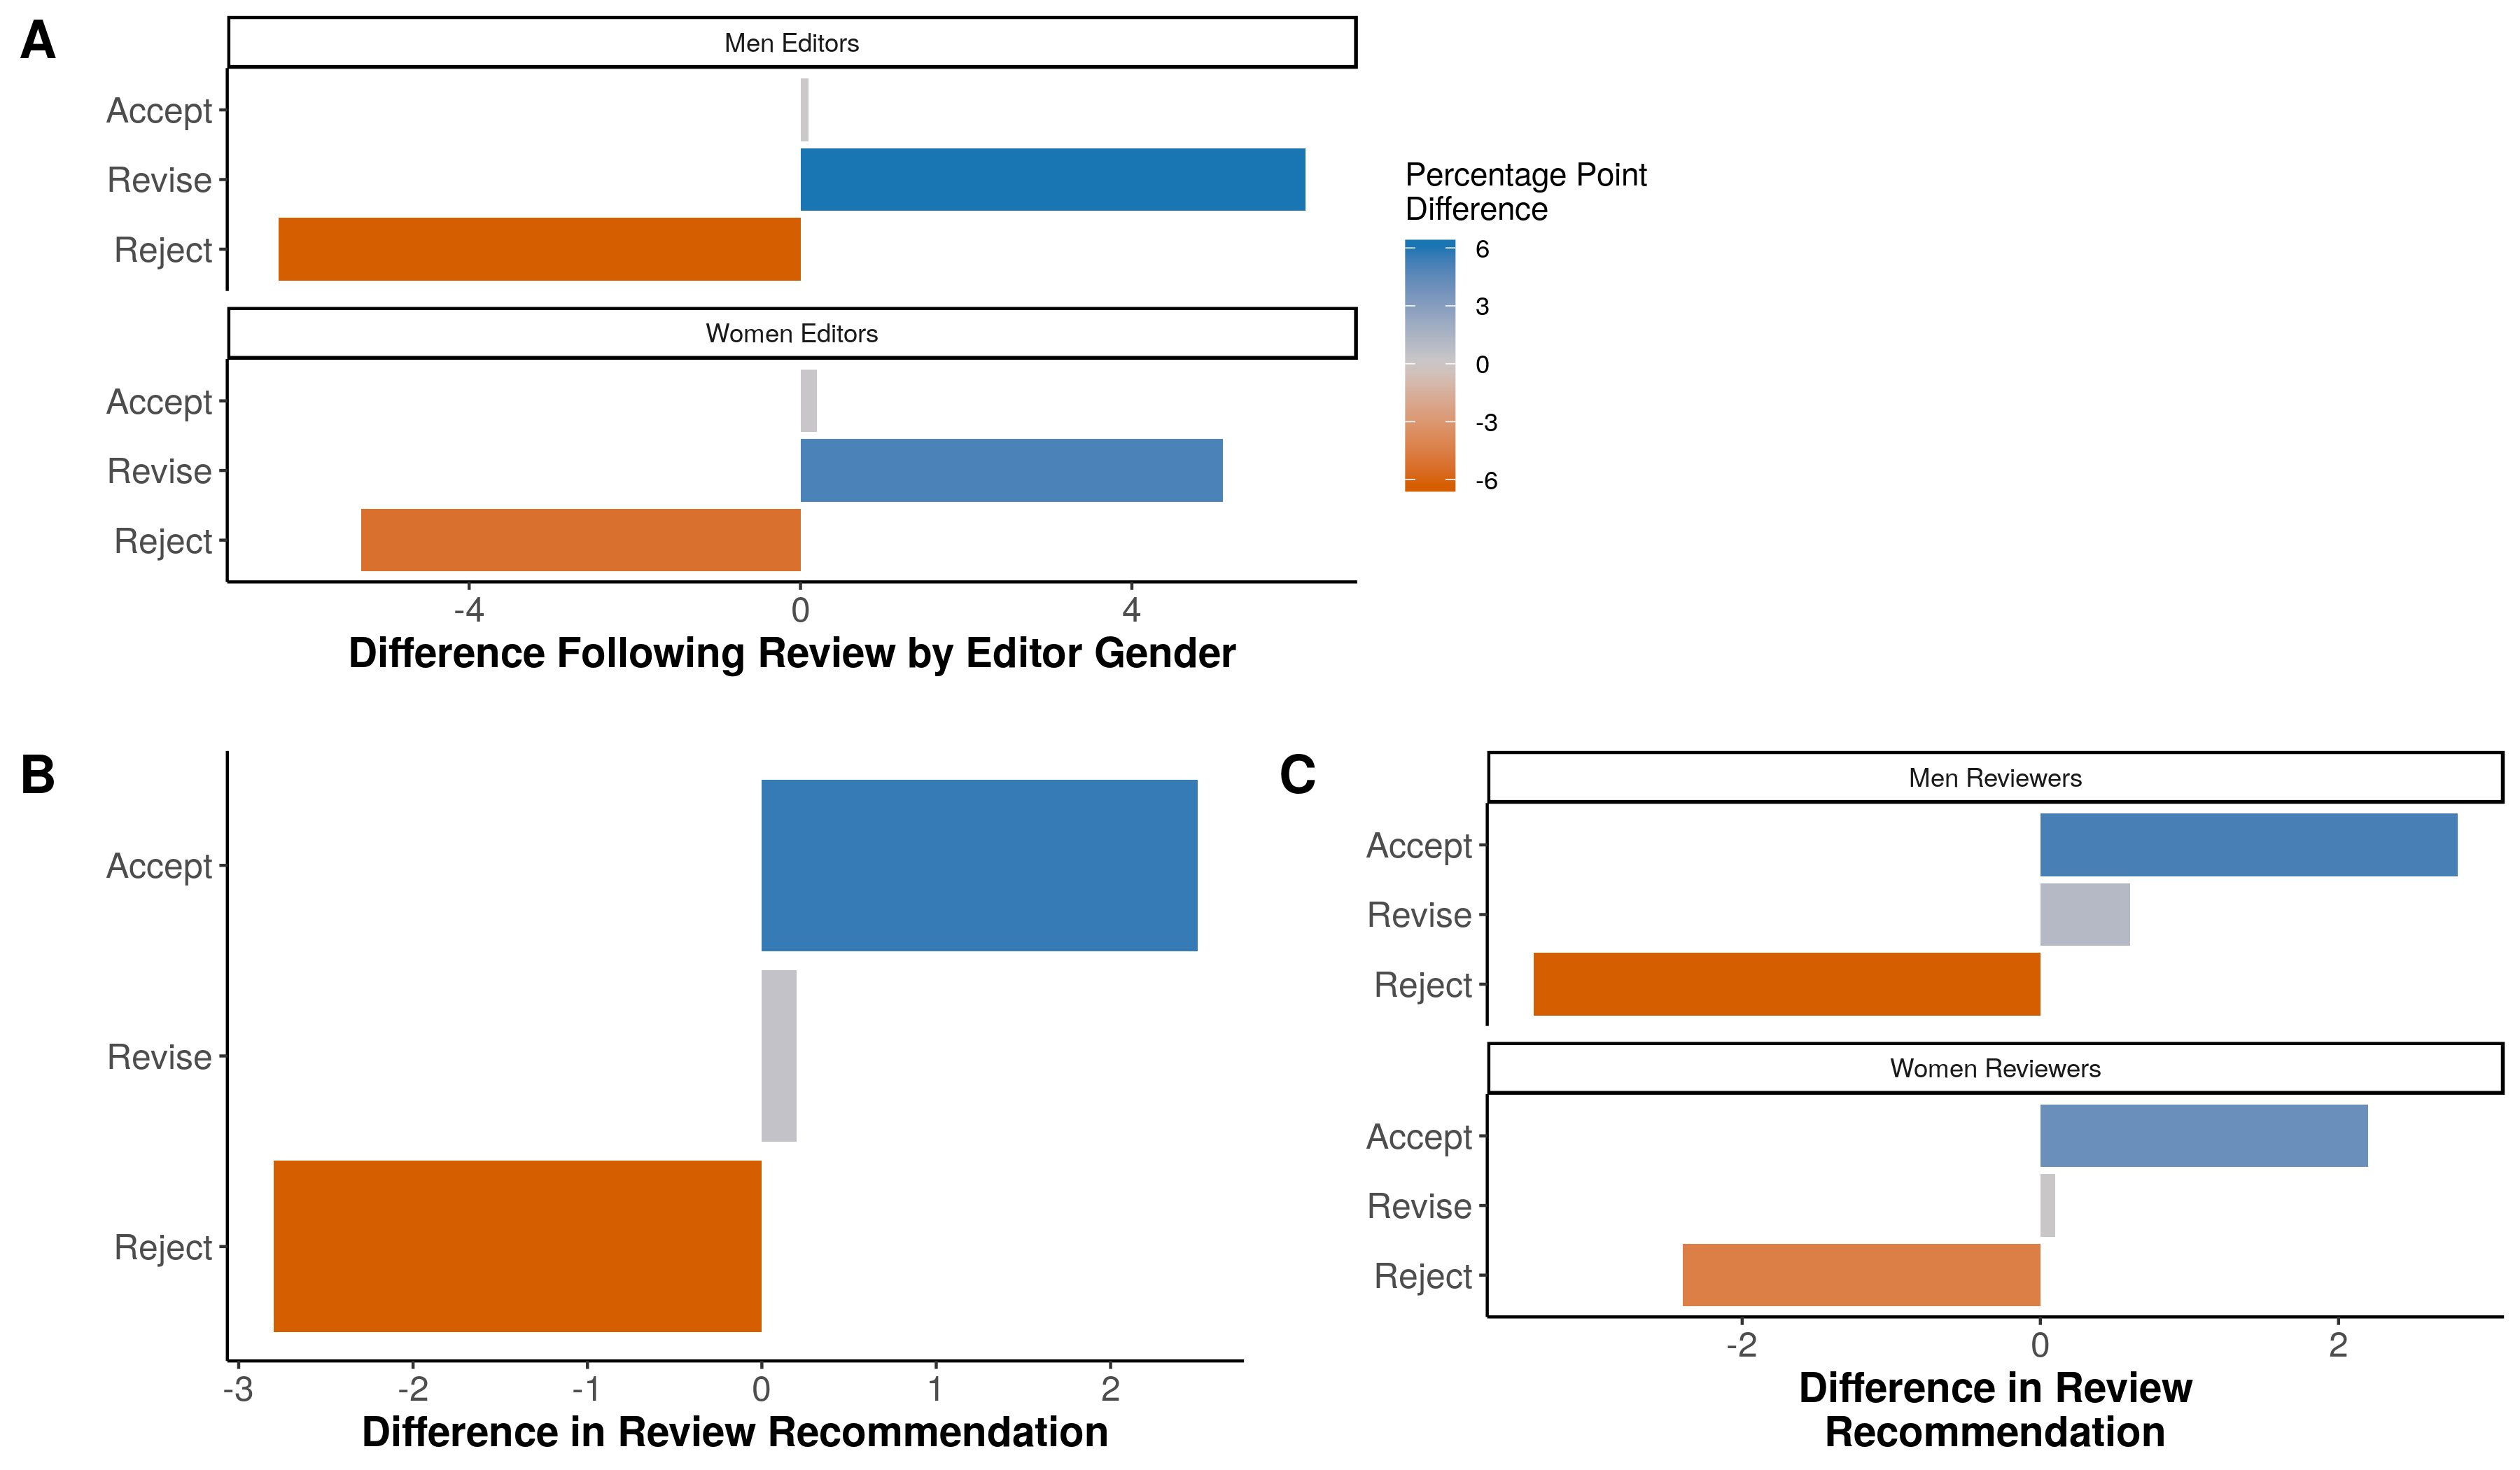
\includegraphics{Figure_5.png}

\textbf{Figure 9. The retention of each gender through the publishing
roles.} All junior (first or middle) authors were split by gender and
tracked through their roles in academic publishing from senior author
(last or corresponding), potential reviewer (considered), reviewer
(accepted), or editor. Color indicates whether (purple) or not (green)
the individual participiated in that role at any point from 2012 to
2018.

The conflation of impact and quality can lead to disparate outcomes for
women who publish in lower impact journals as it negatively impacts
their perceived competency, a bar that women must work harder to achieve
compared to men. Thus the perceived lower impact leads to lower
percieved competency which might in turn affect the likelihood of women
being recognized for their topical expertise. To address this question,
we next asked whether the women who publish at ASM journals as senior
authors are viewed with similar competency to men senior authors.
Indeed, senior authors that are women are less likely to be considered
as reviewers than senior authors that are men, 40 and 50 percent,
respectively.

While the described differences may seem small, they accumulate to
reinforce the decreased representation of women as senior authors seen
in Fig. 4A. To better visualize this and the 1X\% difference in the
proportion of women who are first authors to those who are corresponding
authors we asked the proportions at which women have been retained
through the peer review system at ASM journals. + Get actual proportions
at each stage + seems as if fewer women progress through each stage than
men + greater \# of women (unique indvidiuals) have been suggested as
potential reviewers than \# of women senior authors -- only 1/2 have
actually been reviewers + similar trend for men, except that the
proportions of potential \& accepted seem to be higher - calculate \&
add proportions relative to senior authors

\subsection{Discussion}\label{discussion}

\begin{itemize}
\tightlist
\item
  Summarize results

  \begin{itemize}
  \tightlist
  \item
    Gender

    \begin{itemize}
    \tightlist
    \item
      Women/men/unknown are X percent of authors, reviewers, editors
    \item
      Women/men/unknown are more likely to be repeat authors/submitters
    \item
      M are more likely than W to be suggested as reviewers and are/are
      not used as reviewers at the same proportion
    \item
      M/F editors are more likely to handle multiple manuscripts --
      depends on journal
    \item
      Women are not retained to the same extent as men/unknown
    \item
      These observations do/do not correlate with gender of EiC
    \item
      gap between men \& women peformance, rejection rates
    \item
      women more likely to be editorially rejected or given rejection
      after review
    \item
      that women are more likely to be rejected, have a similar \# of
      versions, and slightly longer times between sub \& pub == women
      are probably given more extensive revisions.
    \end{itemize}
  \end{itemize}
\end{itemize}

The under representation of women as corresponding authors in
publication at ASM journals has negative consequences for their careers
and microbiology. Buckley et al, suggest that being selected as a
reviewer increases visibility of a researcher, which has a direct \&
significant impact on salary. Therefore, the underrepresentation of
women as reviewers hampers their career progression and even their
desire to progress since reviewing also signals adoption of the
researcher into the scientific community (Buckley et al, 2014). This is
supported by Lerback and Hanson who noted that ``It {[}reviewing{]}
provides positive feedback that a scholar is respected and participating
in their field and fosters self-confidence, all of which lead to
increased retention of women.'' (Lerback \& Hanson, 2017) Retention of
women in science is important to the progress of microbiology as a field
since less diversity in researchers limits the diversity of
perspectives, approaches, and thus stunts the search for knowledge. In
addition to boosting productivity and knowledge, more diverse and
equitable organizations are more inclusive and supportive for all
members (Potvin, 2018). It is thus a moral and scientific imperity for
scientific societies and journals, such as ASM, to improve its own
diversity, equity and inclusion efforts. The remainder of this
manuscript will focus on actions that can be taken at multiple levels of
the peer review system to support these efforts.

Certain attributes of biological scientific societies correlate with
increased gender representation at leadership levels (Potvin, 2018).
Using the scientific society ``health checklist'' developed from these
observations, we propose the following suggestions to improve
representation at society journals. First, the development of a visible
mission, vision, or other commitment to equity and inclusion that
includes a non-discrimination clause regarding decisions made by editors
and editors-in-chief. This non-discrimination clause would be backed by
a specific protocol for the reporting of, and responding to, instances
of discrimination and harassment. In the long term, society journals
should begin collecting additional data about authors and gatekeepers
(e.g., race, ethnicity, sexual orientation, gender identity, and
disabilities). Such author data should not be readily available to
journal gatekeepers, but instead kept in a disagreggated manner that
allows the public presentation to track success of inclusive measures
and maintain accountability. Society journals can also impliment
mechanisms to explicity provide support for women and other minority
groups, e.g, by providing APC waivers, reduced copyediting services,
reward inclusive behavior by gatekeepers, encourage women to take up
leadership positions and provide gender-neutral, non-exclusive social
activities.

A common debate when filling leadership positions is whether they should
be representational of the field or aspirational. For instance, since
X\% of corresponding authors to ASM journals are women, X\% of
gatekeepers of a representational leadership would be women. Conversely,
50\% of gatekeepers would be women if the goal were an aspirational
leadership. We argue that whether a goal should be representational or
aspirational depends on the workload and visibility of the position(s).
Since high visibility positions (e.g., editor, EIC) are filled by a
smaller number of individuals that are responsible for recruiting more
individuals into leadership, filling these positions should be done
aspirationally. This allows expansion of the potential reviewer network
and thus recruitment into those positions. These lower visibility
positions (e.g., reviewers) require a greater number of individuals and
should thus be representational of the field to avoid overburdening the
minority population. Outside of leadership appointment, all parties,
journals, gatekeepers, and authors, can help advance women (and other
minority groups) within the peer review system. For instance, authors
can suggest more women as reviewers using ``Diversify'' resources (e.g.,
DiversifyMicrobiology), while reviewers can agree to review for women
editors more often. Editors can rely more on manuscript reference lists
and data base searches than personal knowledge (Fox et al, 2016), and
journals can improve the interactivty and functionality of the peer
review selection software.

Addressing bias during peer review process is a more difficult
challenge, since it is partially the result of accumulated disadvangates
and microaggressions (the actions resulting from implict biases).
Implict bias training for gatekeepers is a start, as might be
double-blinded peer review, a common practice in social sciences. To
support efforts of making peer review more transparent, the review
process could be unblinded following the editor's final decision on a
manuscript. However, these solutions are only bandaids on a deeply
infected wound since both focus on the superficial issue of individuals
instead of the underlying structure of the system that has selected for
the bias at hand.

Reconsidering journal scope and the overall attitude toward
replicatitive and negative results might help address structural
barriers to representation of women in peer review. Significant funds
and staff are required to be competitive in highly active fields (e.g.,
\emph{Clostridium difficile}, HIV), but women are often at a
disadvantage for these resources. As a result, corresponding authors
that are women may be spending their resources at the lesser competitive
fringes of research fields. This has the disadvange of making them seem
``less competent'' to those at the established center of the field. The
decrease in percieved researcher competency and research validity
increase the difficulty to obtain funding and publish in more
traditional journals. Expanding journal scope could provide a home for
these innovative research fields, bolster the field through
reproduciblity, and improve the competentcy demonstration of these
researchers.

Few papers have found disparities between rejection rates of men and
women and to our knowledge, this is the first paper to collectively
examine this issue with either submissions data from 10+ journals or on
the field of microbiology. Critics might argue that the effect size is
too small to really matter or that there are too many unaccounted for
factors to draw conclusions. We acknowledge that these are limitations
of our study along with a limited journal dataset, an absence of
reviewer comments for sentiment analysis, and that many ASM journals
have a narrow focus while the broad scope journals are relatively new.
All of these factors prevent us from generalizing our results across
microbiology as a field. However, the consistency of the trends to
benefit men corresponding authors over women, across all journals
included and literature to-date confirms that this study is highly
relevant for the ASM as a society and offers opportunities to address
both gendered representation in microbiology and systemic barriers to
peer review at our journals.

\subsection{Data and Methods}\label{data-and-methods}

\emph{Data}

All manuscripts handled by ASM journals (e.g., \emph{mBio},
\emph{Journal of Virology}) that received an editorial decision between
January 1st, 2012 and August 31st, 2018 were supplied as XML files by
ASM's publishing platform, eJP. Data were extracted from the XML
documents provided using R statistical software (version 3.4.4) and the
\texttt{XML} package (R citation). Data manipulation was handled using
the \texttt{tidyverse}, \texttt{lubridate}, and \texttt{xml2} packages
for R. Variables of interest included: the manuscript number assigned to
each submission, manuscript type (e.g., full length research, erratum,
editorial), category (e.g., microbial ecology), related (previously
submitted) manuscripts, versions submitted, dates (e.g., submission,
decision), author data (e.g., first, last, and corresponding authorship,
total number of authors), reviewer data (e.g., reviewer score,
recommendation, editor decision), and person data (names, institutions,
country) of the editors, authors, and reviewers.

For this analysis, only original, research-based manuscripts were
included, e.g., long- and short-form research articles, New-Data
Letters, Observations, Opinion/Hypothesis articles, and Fast-Track
Communications.

It is common practice at ASM journals for manuscripts whose reviewers
recommend extensive experimental revisions be given a decision of
``reject with resubmission encouraged''. If resubmitted, the authors are
asked to note the previous (related) manuscript and the resubmission is
assigned a new manuscript number. Multiple related manuscripts were
tracked together by generating a unique grouped manuscript number based
on the recorded related manuscript numbers. This grouped manuscript
number served multiple purposes including: tracking a single manuscript
through multiple rejections or transfers between ASM journals and to
avoid duplicate counts of the same authors for the same manuscript.

Data were visualized using the \texttt{ggplot}, \texttt{scales},
\texttt{RColorBrewer}, and \texttt{ggalluvial} packages for R.

\emph{Bias analysis and presentation}

\emph{Logistic regression and clustering}

\emph{Gender prediction and assignment}

The gender assignment API genderize.io was used to predict an
individual's gender based on their given names, and country where
possible. The genderize.io platform uses data gathered from social media
to predict gender based on given names with the option to include an
associated language or country to enhance the odds of successful
prediction. Since all manuscripts are submitted in English, precluding
language association for names with special characters, names were
standardized to ASCII coding (e.g., ``José'' to ``Jose''). We next
matched each individuals country against the list of X country names
accepted by genderize.io. Using the \texttt{GenderGuesser} package for
R, all unique given names associated with an accepted country were
submitted to the genderize.io API and any names returned without a
predictive assignment of either male or female were resubmitted without
an associated country. All predictive assignments of either male or
female are returned with a probability match of 0.50 or greater. The
predicted genders of all given names (with and without an associated
country) whose probabilities were greater or equal to our arbitrary
success cut off of 0.65 were used to assign predicted gender to the
individuals in our dataset. Predicted genders were assigned to
individuals in the following order: first names and country, first
names, middle names and country, middle names (Supplemental Fig. 1). The
presenting gender (man/woman) of editors and senior editors in our
dataset was hand validated using Google where possible.

We recognize that biological sex (male/female) is not always equivalent
to the gender that an individual presents as (man/woman), which is also
distinct from the gender(s) that an individual may self-identify as. For
the purposes of this manuscript, we choose to focus on the presenting
gender (man/woman/unknown) based on their first names and/or appearance
(for editors). In the interest of transparency, we include those
individuals whose names don't allow a high degree of confidence for
gender assignment in the ``unknown'' category of our analysis.

\emph{Validation of gender prediction}

We first validated the algorithm using a set of 3265 names whose gender
had been hand-coded based on appearance and were generously provided to
us by \_\_\_ (preprint cite). The names were supplied to the genderize
algorithm both with and without the accompanying country data. The data
returned include the name, predicted gender (male, female, na), the
probability of correct gender assignment (ranging from 0.5 to 1.0), and
the number of instances the name and gender were associated together (1
or greater). The genderize algorithm returned gender predictions for
2899 when first names were given and 2167 when country data was also
supplied (732 names were associated with countries unsupported by
genderize).

Sensitivity and specificity, are measurements of the algorithm's
tendency to return correct answers instead of false positives (e.g., a
man incorrectly gendered as a woman) or false negatives (e.g., a woman
incorrectly gendered as a man). The closer these values are to 1, the
smaller the chance that the algorithm will return the correlating false
response. Accuracy is a composite measure of the algorithm's ability to
differentiate the genders correctly. These measurements were calculated
from the datasets (with and without country data supplied) at three
different probability threshold cutoffs: the default genderize (0.5), a
probability threshold of 0.85 (0.85), and a modified probability of
0.85, which factors in the number of instances returned
(pmod0.85)(citations).

At the 0.5 threshold, the dataset returned a sensitivity of 0.8943 and
specificity of 0.9339 for an accuracy of 0.911, compared to a marginally
higher accuracy of 0.9146 for the dataset where country data were
included (Supplemental Table 1). Generally speaking, the accuracy
increases as the threshold increases along with slight trade offs
between sensitivity and specificity. For the purposes of our analysis,
we opted to use the pmod0.85 threshold moving forward (Supplemental
Table 1, in bold).

To understand the extent of geographic bias in our gender assignment
against regions and languages with genderless naming conventions, or
that lack social media for incorporation into the genderize algorithm,
we compared the number of names predicted without associated country
data to when country data was also supplied. In our test dataset, the
top five countries associated with names were United States, Germany,
United Kingdom, France, and China and the countries with the highest
proportion of un-predicted genders when country data were supplied are
Cambodia, Iceland, Indonesia, Ireland, and Mexico, where the maximum
number of names supplied ranged from 1 to 15. To determine the impact of
each country towards the overall percentage of names whose genders were
not predicted (27.14\%), we found the difference between the percent of
names unpredicted for each country and the overall percentage,
multiplied by the proportion of observations from that country to the
total observations and finally divided by the overall percentage of
unpredicted names (Supplemental Fig. 2). The top five countries with the
greatest impact on unpredicted names, and thus the countries receiving
the most negative bias from genderize were Canada, China, Ireland,
Belgium, and Sweden (Supplemental Fig. 3). These data suggest that there
is likely some bias against countries with gender-neutral naming
conventions (China), and indicates the stringency with which the
algorithm applies gender to names that are accompanied by country data.
For instance, strongly gendered names such as Peter and Pedro were not
assigned gender when associated with Canada.

We next applied the genderize algorithm at the pmod0.85 threshold to our
journals dataset and tested its validity on a small portion. All first
names collected from our dataset were submitted to genderize both with
and without country data. Only those predictions whose pmod were
equivalent or greater than 0.85 were carried to the next step. The
predicted genders were assigned to individuals in the following order:
first names and country, first names, middle names and country, middle
names. Given the relatively small number of editors and senior editors
in our dataset, the presenting gender (man/woman) of editors and senior
editors in our dataset was hand-validated using Google where possible.
Of the 1072 editor names, 938 were predicted by genderize for an
accuracy of 0.9989339, thus increasing our confidence in the gender
predictions where made.

In our full dataset, the five countries with the most individuals were
United States, China, Japan, France, and Germany and the countries with
the highest proportion of un-predicted genders were Burundi, Chad,
Kingman Reef, Korea (North), Democratic People's Republic of, and
Maldives, where the maximum number of names supplied ranged from 1 to 4.
Proportionally, fewer names in our full dataset were assigned gender
than in our validation dataset (40.01\% unpredicted versus 27.14\%
unpredicted, respectively). Since adjusting the workflow to predict the
gender of names both with and without country data, the countries
receiving the most negative bias from genderize were China, Japan,
Korea, Republic of, India, Taiwan, Province of China (Supplemental Fig.
4). These data indicate what we previously predicted, that the genderize
algorithm has bias against countries with gender-neutral naming
conventions.

\emph{Code availability}

The code for all analysis steps, including an Rmarkdown version of this
manuscript, is available at
\url{https://github.com/SchlossLab/Hagan_Gender_mBio_2019/}

\subsection{References}\label{references}


\end{document}
